\documentclass[a5paper]{article}
\usepackage[a5paper, top=8mm, bottom=8mm, left=8mm, right=8mm]{geometry}

\usepackage{polyglossia}
\setdefaultlanguage[babelshorthands=true]{russian}

\usepackage{fontspec}
\setmainfont{FreeSerif}
\newfontfamily{\russianfonttt}[Scale=0.7]{DejaVuSansMono}

\usepackage[font=scriptsize]{caption}

\usepackage{amsmath}
\usepackage{amssymb,amsfonts,textcomp}
\usepackage{color}
\usepackage{array}
\usepackage{hhline}
\usepackage{cite}
\usepackage{textcomp}

\usepackage[hang,multiple]{footmisc}
\renewcommand{\footnotelayout}{\raggedright}

\PassOptionsToPackage{hyphens}{url}\usepackage[xetex,linktocpage=true,plainpages=false,pdfpagelabels=false]{hyperref}
\hypersetup{colorlinks=true, linkcolor=blue, citecolor=blue, filecolor=blue, urlcolor=blue, pdftitle=1, pdfauthor=, pdfsubject=, pdfkeywords=}

\newlength\Colsep
\setlength\Colsep{10pt}

\usepackage{tabu}

\usepackage{graphicx}
\usepackage{indentfirst}
\usepackage{multirow}
\usepackage{subfig}
\usepackage{footnote}
\usepackage{minted}

\newcommand{\todo}[1] {
\begin{center}\textcolor{red}{TODO: #1}\end{center}
}

\newcommand{\attribution}[1] {
    \vspace{-5mm}\begin{flushright}\begin{scriptsize}%\textcolor{gray}
    {\textcopyright\, #1}\end{scriptsize}\end{flushright}
}

\sloppy
\pagestyle{plain}

\title{Лекция 8: Поведенческие шаблоны}
\author{Юрий Литвинов\\\small{y.litvinov@spbu.ru}}
\date{26.10.2021}

\begin{document}

\maketitle
\thispagestyle{empty}

\section{Паттерн <<Строитель>>}

\subsection{Мотивирующий пример}

Начнём с одного порождающего паттерна, который не поместился в предыдущую лекцию. Предположим, мы хотим сделать утилиту, которая бы читала текст в некотором формате (допустим, .rtf) и конвертировала бы его в другой формат (например, TeX, .docx, plain text и т.д.). .rtf содержит информацию о структуре текста и его форматировании. Мы не хотим писать несколько разных конвертеров, а хотим считать .rtf один раз и конвертировать его в разные целевые форматы, причём не строя какого-то внутреннего представления (поскольку формат довольно простой и усложнять систему не хотелось бы).

На помощь приходит паттерн <<Строитель>>:

\begin{center}
    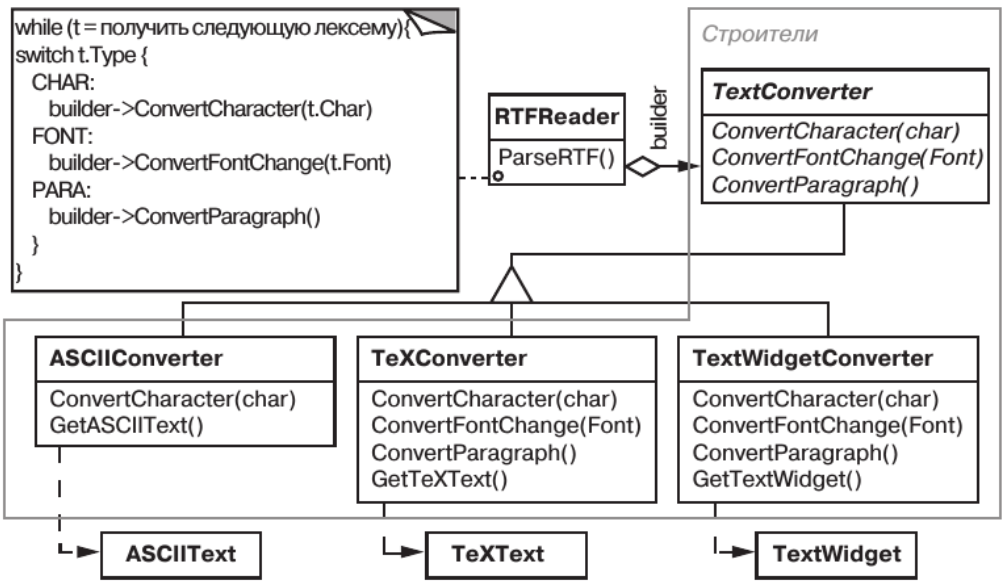
\includegraphics[width=0.9\textwidth]{textConverter.png}
    \attribution{Э. Гамма и др., Приемы объектно-ориентированного проектирования}
\end{center}

Есть класс RTFReader, который занимается разбором .rtf-документа. Он параметризуется одним из видов конвертеров, каждый из которых принимает элементы документы и что-то с ним делает. Например, ASCIIConverter может просто каждый переданный символ добавлять к строке, а команды форматирования просто игнорировать. Задача RTFReader --- последовательно <<скормить>> весь документ установленному в него конвертеру. Забрать результат потом можно с помощью метода Get-что-то-там у конвертера (они у всех разные).

Теперь, во-первых, процесс конвертации строго детерминирован и управляется централизованно в RTFReader, во-вторых, конвертеры легко менять, поскольку они реализуют один интерфейс и RTFReader-у всё равно, с кем из них работать. И реализовывать конвертеры просто, поскольку им не надо заботиться о разборе документа, и пони получают документ маленькими частями.

\subsection{Строитель (Builder), общая структура}

Эта идея обобщается до паттерна <<Строитель>>:

\begin{center}
    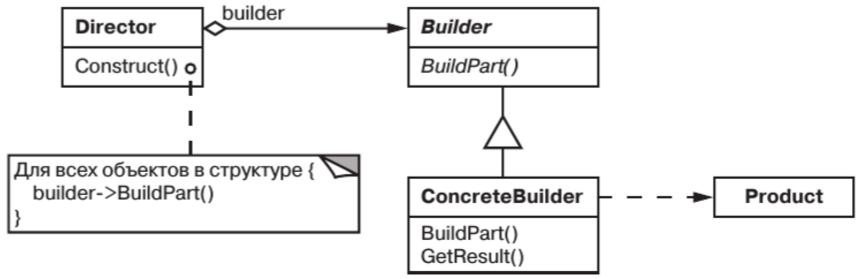
\includegraphics[width=0.85\textwidth]{builder.png}
    \attribution{Э. Гамма и др., Приемы объектно-ориентированного проектирования}
\end{center}

Класс Director (<<распорядитель>> в русскоязычной литературе) параметризуется Builder-ом и отвечает за то, чтобы передавать Buider-у части строящегося объекта (RTFReader в нашем примере). Builder --- интерфейс или абстрактный класс, имеющий методы, принимающие разные виды частей. Конкретный Builder реализует интерфейс Builder-а и постепенно строит Product. Когда процесс закончен, тот, кто заказывал строительство (Director или тот, кто создал Director и Builder), может получить Product с помощью метода GetResult().

\subsection{Детали реализации}

В реализации самое важное --- это определить интерфейс Builder так, чтобы любой конкретный строитель получал все необходимые части и мог эффективно строить Product. Обратите внимание, что GetResult() не является частью интерфейса Builder, и это важно по следующим причинам:

\begin{itemize}
    \item разные ConcreteBuilder-ы могут строить разные Product-ы, никак не связанные иерархией наследования;
    \item Director-у не нужно знать про продукты вовсе, он просто обходит структуру и отдаёт её части Builred-у; что именно строится, его не волнует;
    \item помимо Director и Builder, по всей видимости, где-то есть клиент, который и заказывает стройку --- клиент создаёт Builder, создаёт Director, передавая ему Builder, и запускает Construct() у Director-а. По окончании строительства у клиента всё ещё есть ссылка на конкретный Builder, потому что он же его и создал. Соответственно, клиент может забрать результат, вызвав GetResult().
\end{itemize}

Ещё иногда стоит Builder делать всё-таки абстрактным классом, а не интерфейсом, чтобы сделать его методам пустые реализации по умолчанию\footnote{Недавно в современных языках возникла мода на реализации по умолчанию для методов интерфейсов --- изначально это появилось в Java как средство обеспечения обратной совместимости при расширении интерфейсов (код, который не знает про новые методы интерфейса, может благодаря реализации по умолчанию их не реализовывать, соответственно, не надо перекомпилировать миллионы строк кода). Потом этот механизм начали неправильно использовать, и вот, интерфейс и абстрактный класс теперь почти неотличимы.}. Это мы использовали в мотивирующем примере для реализации ASCIIConverter-а, которому большая часть тегов RTF-документа (относящихся к форматированию) не интересна в силу природы конструируемого объекта.

В реальной жизни паттерн <<Строитель>> встречается довольно часто --- например, в любой нормальной стандартной библиотеке есть класс StringBuilder или его аналоги. Это класс, нужный для конкатенации нескольких строк в одну. Наивное решение:

\begin{minted}{csharp}
    var result = ""
    foreach (var string in stringList) {
        result += string;
    }
\end{minted}

Оно на самом деле квадратично по времени и по памяти, хотя выглядит линейным. Дело в том, что при каждой конкатенации выделяется память под хранение результирующей строки и обе конкатенируемые строки копируются в выделенную область. Потом сборщик мусора может подчистить промежуточные результаты, но это тоже занимает кучу времени. Если мы хотим сконкатенировать тысячу коротких строк, делать так --- очень плохая идея.

На помощь приходит StringBuilder. У него есть метод, позволяющий добавить строку к списку конкатенируемых строк, и метод, позволяющий получить результат. Добавление строки просто кладёт её в список, за константное время. Получение результата --- это пробежаться по списку, узнать длины всех строк, сложить (за линейное относительно количества строк время), сделать \emph{одно} выделение памяти для хранения результата, и скопировать туда последовательно строки из списка (за линейное относительно количества символов время).

В этом примере StringBuilder --- это, очевидно, Builder, а код, который его использует, выступает в роли и Director-а, и клиента одновременно.

Второй пример --- это подсистема работы с графами известной библиотеки Guava\footnote{Если вы знакомы с C++, Guava для Java --- примерно как Boost для C++. Страница Google Guava на GitHub: \url{https://github.com/google/guava} (дата обращения: 28.08.2021г).}. Там графы бывают трёх видов: Graph (граф в классическом математическом понимании, множество узлов и бинарное отношение на этом множестве, представляющее рёбра), ValueGraph (граф с метками на рёбрах) и Network --- то, что у нас обычно называют мультиграфом (или псевдографом): граф с параллельными рёбрами (то есть где ребро не просто элемент отношения, а полноценный объект). Это на самом деле интерфейсы, а конкретная реализация для них выбирается на основе ожиданий пользователя --- если граф маленький, то обычная матрица смежности будет работать быстро и качественно, если большой разреженный, то надо придумывать ещё что-то. Про конкретные реализации клиент в принципе не знает, а выбирает реализацию для него Builder:

\begin{minted}{java}
MutableNetwork<Webpage, Link> webSnapshot = 
        NetworkBuilder.directed()
    .allowsParallelEdges(true)
    .nodeOrder(ElementOrder.natural())
    .expectedNodeCount(100000)
    .expectedEdgeCount(1000000)
    .build();
\end{minted}

Этот код создаёт реализацию мутабельного мультиграфа, у которого направленные рёбра, при этом ожидается порядка ста тысяч вершин и миллиона рёбер. Когда мы вызываем build, строитель смотрит на переданные ему параметры, выбирает подходящую реализацию и создаёт граф. Такой подход позволяет авторам Guava менять существующие и внедрять новые реализации графов совершенно незаметно для клиентского кода, а прикладным программистам --- не учить теорию про представление разреженных матриц.

На самом деле, этот приём --- один из самых частых случаев использования Builder-а на практике --- не чтобы, как в книжке, долго создавать сложные структуры, а как продвинутый конструктор с возможностью передачи параметров постепенно, проверки параметров и подстановки значений по умолчанию, и выбора типа времени выполнения создаваемого объекта. Паттерн Builder очень рекомендуется использовать, если у вас у класса уже несколько конструкторов и вы начинаете путаться в их параметрах.

\section{Паттерн <<Наблюдатель>>}

\subsection{Мотивирующий пример}

Паттерн <<Наблюдатель>> используется настолько часто, что и мотивирующий пример особо не нужен, но всё же: положим, у нас есть некоторые данные и приложение, позволяющее их показывать и редактировать. Причём, в разных форматах: в виде таблицы, в виде столбчатой или круговой диаграммы. И мы, естественно, хотим поддерживать консистентность этих данных --- чтобы если мы поменяем табличное представление, диаграммы бы сами тут же перерисовались, или если мы поменяем что-то на диаграмме, поменялось бы что-то и в таблице. Это можно реализовать примерно так:

\begin{center}
    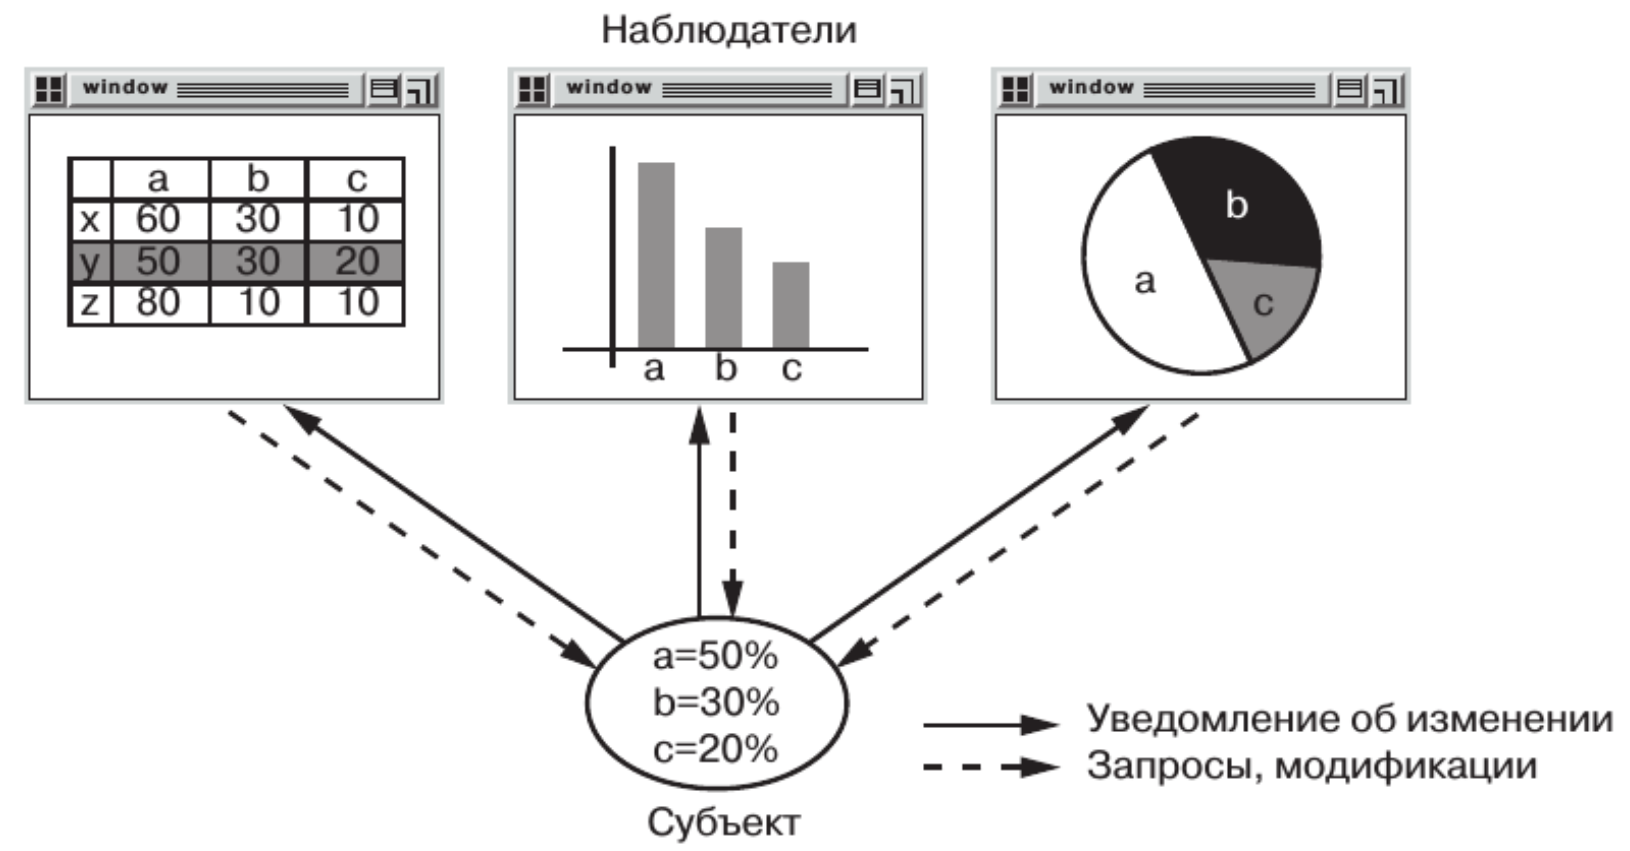
\includegraphics[width=0.8\textwidth]{observerExample.png}
    \attribution{Э. Гамма и др., Приемы объектно-ориентированного проектирования}
\end{center}

Данные хранятся в объекте <<Субъект>> (в реальной жизни это может быть Data Access Layer поверх СУБД, например). Разные представления реализуются в объектах-видах, которые знают про субъект и могут его модифицировать. Субъект знает про то, что виды существуют, но не знает про них никаких подробностей (чтобы не было совсем уж круговой зависимости). Когда какой-то из видов (да на самом деле не обязательно вид, кто угодно) меняет данные в субъекте, он проходится по списку видов и каждому говорит <<данные изменились, обновись>>. Вид перечитывает относящиеся к нему данные из субъекта и обновляется.

\subsection{Наблюдатель (Observer), общая структура}

Эта схема обобщается до паттерна <<Наблюдатель>>, который структурно устроен вот так:

\begin{center}
    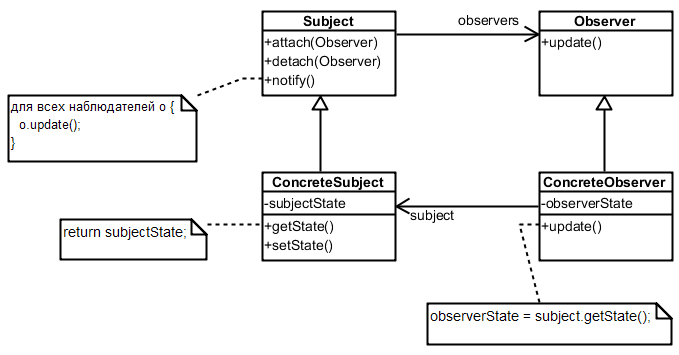
\includegraphics[width=0.9\textwidth]{observer.png}
\end{center}

Subject --- это штука, которая генерирует события, за которыми можно наблюдать. В классическом варианте это абстрактный класс, который содержит список наблюдателей, позволяет регистрировать наблюдателей и вызывать их нотификацию. ConcreteSubject наследуется от него и часто, хотя и необязательно, хранит в себе данные. Observer --- это интерфейс наблюдателя, про него знает Subject. Как правило, интерфейс очень простой, содержит всего один метод (или совсем немного методов), только для того, чтобы Subject мог его нотифицировать. Всё интересное происходит в ConcreteObserver, который уже на самом деле реагирует на событие в Subject-е. ConcreteObserver может знать про свой ConcreteSubject, может запрашивать его состояние и при необходимости использовать его при обработке нотификации.

Паттерн позволяет реализовать событийную схему и реактивное программирование там, где язык этого не поддерживает (а если язык поддерживает, то на самом деле реализует <<Наблюдатель>> сам). Событийная модель позволяет полностью отвязать генератор событий от тех, кто реагирует на события, существенно понизив связность и, обычно, повысив переисползуемость. Событийная модель как бы разворачивает схему управления --- обычно цикл обработки событий явно вызывает обработчики, а тут генератор событий никого не вызывает, просто говорит, что событие произошло. Если на него кто-то подписан, событие будет обработано, если нет, то ну и ладно. В этом курсе ещё будет про архитектурные преимущества и недостатки такого подхода, когда будут обсуждаться архитектурные стили.

\subsection{Детали реализации}

В плане реализации важно понимать, что в современных языках часто этот паттерн реализовывать не нужно, он уже <<встроен>> в язык. Например, C\# имеет ключевое слово event, которое делает в точности то, что делает <<Наблюдатель>> --- декларирует список наблюдателей, возможность подписаться и отписаться, и нотифицировать наблюдателей о событии, причём это всё очень удобно. В C++ есть библиотека Qt, которая во многом построена вокруг событийной схемы, реализуемой с помощью языковых расширений C++ --- механизма сигналов и слотов и функции connect. Поскольку даже современный C++ события не поддерживает, Qt требуется продвинутый препроцессинг с кодогенерацией, чтобы реализовать эти возможности, и оно не так удобно, как в C\#, но тоже вполне работает. В Java ничего такого нет, но есть библиотечные интерфейсы, предназначенные для использования в качестве наблюдателей и, на самом деле, языковые особенности типа нестатических вложенных классов наличествуют в Java отчасти как раз для удобной поддержки паттерна <<Наблюдатель>>.

Субъекты могут быть устроены хитрее, чем на диаграмме выше. Например (и это очень характерный пример для паттерна), в оконных библиотеках в качестве субъекта выступают элементы управления, а в качестве событий, за которыми можно наблюдать --- события от пользователя и операционной системы. С каждым элементом управления могут произойти десятки (иногда более сотни) разных событий, и на каждое могут подписаться разные наблюдатели. Поэтому часто для того, чтобы не хранить сотню пустых списков, наблюдатели хранятся в более продвинутых структурах данных, например, хеш-таблице, которая отображает тип события на список наблюдателей, на него подписанных. Если никто не подписан, хеш-таблица пуста (мы можем вообще хранить только один null в таком случае), если кто-то подписался на одно-два события, в хеш-таблице хранятся только эти наблюдатели. Так делает библиотека WPF\footnote{Windows Presentation Foundation, \url{https://docs.microsoft.com/en-us/dotnet/desktop/wpf/?view=netdesktop-5.0} (дата обращения: 01.09.2021).}, в языке C\# есть даже поддержка для произвольных обработчиков подписывания-отписывания наблюдателей, которые, собственно, и позволяют реализовать такие ухищрения.

Да и сами наблюдатели могут быть устроены хитрее --- в частности, наблюдать за несколькими субъектами одновременно. И так они часто и делают --- например, один обработчик клика на кнопку в оконном интерфейса может следить сразу за несколькими кнопками. В этом случае необходим способ идентифицировать субъект, который послал нотификацию. Поэтому, например, в .NET любой обработчик события по соглашению всегда первым аргументом принимает ссылку на объект, который послал событие. В Qt в обработчике события доступна функция sender(), которая возвращает указатель на объект, пославший сигнал. В любом случае, об этом стоит заранее подумать.

Ещё важный архитектурный вопрос --- кто инициирует нотификацию. Из всего, что говорилось выше, можно сделать вывод, что это всегда делает субъект, когда в нём что-то меняется. Однако часто это неэффективно --- если субъект подвергается серии из большого количества мелких правок, посылать нотификацию на каждую может быть слишком трудозатратно. В таком случае notify() у субъекта делают публичным методом, который вызывает тот, кто модифицирует субъект, когда он закончил серию правок. Например, при редактировании таблицы часто может возникнуть потребность поменять данные в целом столбце --- из-за каждой ячейки перерисовывать все диаграммы как-то не очень. Или, опять-таки, в библиотеках для оконных интерфейсов механизм размещения элементов на форме (<<лейаут>>) обычно не работает во время массового создания элементов, чтобы не перераскладывать их каждый раз. Когда форму создали, лейаут вызывается один раз, в конце, и дальше уже автоматически следит за изменением размеров.

Не стоит забывать про то, что субъекты хранят ссылки на наблюдателей, чтобы извещать их о событиях. В языках, где работа с наблюдателями сделана удобно (например, в C\#) это может привести к внезапным утечкам памяти --- подписаться и забыть отписаться, так делают даже опытные программисты. В языках без сборки мусора --- например C++ --- забыть отписаться и удалить наблюдатель --- отличный способ получить Segmentation Fault/Access Violation, который очень сложно отладить (потому что <<плохое>> событие может происходить очень редко).

Ещё один подводный камень --- это что при отправке нотификации субъект должен полностью завершить обновление своего состояния. Это кажется очевидным соображением, однако при наследовании от субъекта это легко случайно нарушить. Например:

\begin{minted}{csharp}
public abstract class Subject
{
    private int data1 = 0;
    private int data2 = 0;

    public void Update()
    {
        data1 = 1;
        DoUpdate();
        data2 = 1;
        Notify(this);
    }

    protected void Notify(object sender)
    {
        ...
    }

    protected abstract void DoUpdate();
}

public class ConcreteSubject
{
    private int data3 = 0;

    public void DoUpdate()
    {
        data3 = 1;
        Notify(this);  // Ну а что, мы же изменились
        // Наблюдатели увидят data2 == 0, что может быть некорректно, а потом получат 
        // ещё одну нотификацию
    }
}
\end{minted}

Эта проблема тут очевидна, но если у вас сотни строк кода в каждом классе и десяток разных видов событий, уследить за всем становится уже проблематичнее (по крайней мере, автор сталкивался с такими проблемами в реальной практике и даже иногда создавал их). На помощь может прийти паттерн <<Шаблонный метод>> (про который чуть ниже) и архитектурное ограничение, что потомок никогда никого не нотифицирует. И вообще, крайне полезно документировать, кто какие события бросает. Кстати, в C\# нотифицировать о событии может только сам субъект, в некоторых других системах (например, Qt) --- кто угодно. Идеологически первый подход правильнее, бросание событий от имени субъекта без ведома субъекта может радикально всё запутать.

Ещё есть выбор между вариантами передачи данных (как в паттерне <<Стратегия>>) --- либо субъект рассылает вместе с нотификацией информацию о том, что именно в нём изменилось (push- схема), либо субъект просто говорит, что в нём что-то изменилось, а наблюдатели потом спрашивают у него, что именно (pull-схема). Первый подход хорош тем, что наблюдателям не надо знать подробностей устройства субъекта, а субъекту --- иметь отдельный интерфейс для доступа наблюдателей к своему состоянию, второй --- тем, что наблюдатели не получают кучи не нужных им данных и не надо менять сигнатуру notify() (и обновлять его в каждом наблюдателе), как только появляются какие-то новые данные. На схеме паттерна изображён второй способ, на практике бывает по-разному (например, .NET предпочитает первый, но хитро --- упаковывает параметры в класс, и если появляются новые параметры, то появляется новый класс-наследник, так что наблюдатели, которым эти параметры не интересны, могут продолжать пользоваться интерфейсом предка. Кому интересно, погуглите EventArgs --- этот приём, кстати, ещё встретится нам в паттерне <<Цепочка ответственности>>). Бывают вообще промежуточные результаты, например, в Qt-шной реализации архитектурного паттерна Model-View-Controller модель сообщает наблюдающим за ней видам, что она поменялась, и какая конкретно её часть поменялась, но не сообщает новые данные. Виды делают запрос к модели, как при pull-схеме, но точно знают, про какие элементы модели спрашивать (эта информация им рассылается по push-схеме) --- что позволяет видам игнорировать изменения в модели, которые их заведомо не касаются, и при этом не получать кучу ненужных данных.

В принципе, возможно применение и более хитрой системы маршрутизации сообщений от субъектов к наблюдателям. Как правило, это полезно в распределённых или сильно реактивных системах. Реализуется наличием некоторого менеджера сообщений (паттерн <<Посредник>>), который может хранить сообщения, доставлять разным адресатам, гарантировать их доставку, фильтровать и преобразовывать. Примеры таких систем --- библиотека Rx.NET, которая расширяет модель event-ов C\# как раз продвинутыми методами диспетчеризации сообщений (и вообще, позволяет смотреть на сообщения не как на нечто одномоментное, а как на бесконечный поток данных, с которым можно работать, как с любой нормальной коллекцией --- выполнять Map, Filter и подобные функции), система событий F\# (которая на самом деле очень-очень близка Rx.NET), очереди сообщений (например, RabbitMQ, но их только популярных чуть ли не десяток), менеджеры стримов сообщений (например, Apache Kafka). Правда, если дело дошло до Kafka и прочей тяжёлой артиллерии, речь идёт уже не о паттерне <<Наблюдатель>>, а о событийно-ориентированных архитектурных стилях.

\section{Паттерн <<Шаблонный метод>>}

\subsection{Мотивирующий пример}

Помнится, в паттерне <<Фабричный метод>> мы обсуждали ситуацию, когда у нас есть редактор и несколько разных видов документов, с которыми он может работать. И с помощью фабричного метода мы научились удобно создавать разные виды документов так, чтобы редактор мог единообразно с ними работать и даже не знать, что за документы бывают. 

Пойдём дальше. Создали мы документ, но, наверное, элементарные действия, типа открытия документа, могут быть для каждого документа свои, и вместе с тем есть какой-то общий алгоритм, которому все документы подчиняются. Например, чтобы открыть документ, надо запросить местоположение документа (и это может быть файл на диске, а может быть документ в облаке, в зависимости от вида документа), проверить, что мы можем его открыть, вызвать переопределяемый для каждого вида документа hook, что мы его вот-вот сейчас откроем, и, собственно, открыть (опять-таки, специфичным для каждого документа образом). Если мы для каждого документа отдельно будем реализовывать эту последовательность событий, то наверняка для кого-то сделаем что-то не так, и оно будет неконсистентно, а может, и вовсе неправильно.

<<Шаблонный метод>> (не путать с фабричным методом!) предлагает решение (которое на самом деле является просто развитием идеи фабричного метода): давайте мы в базовом классе опишем алгоритм в терминах некоторых абстрактных операций, а в наследниках определим эти операции уже для конкретного документа --- примерно как в фабричном методе, там была абстрактная операция создания, определяемая в потомках. Получится что-то такое:

\begin{center}
    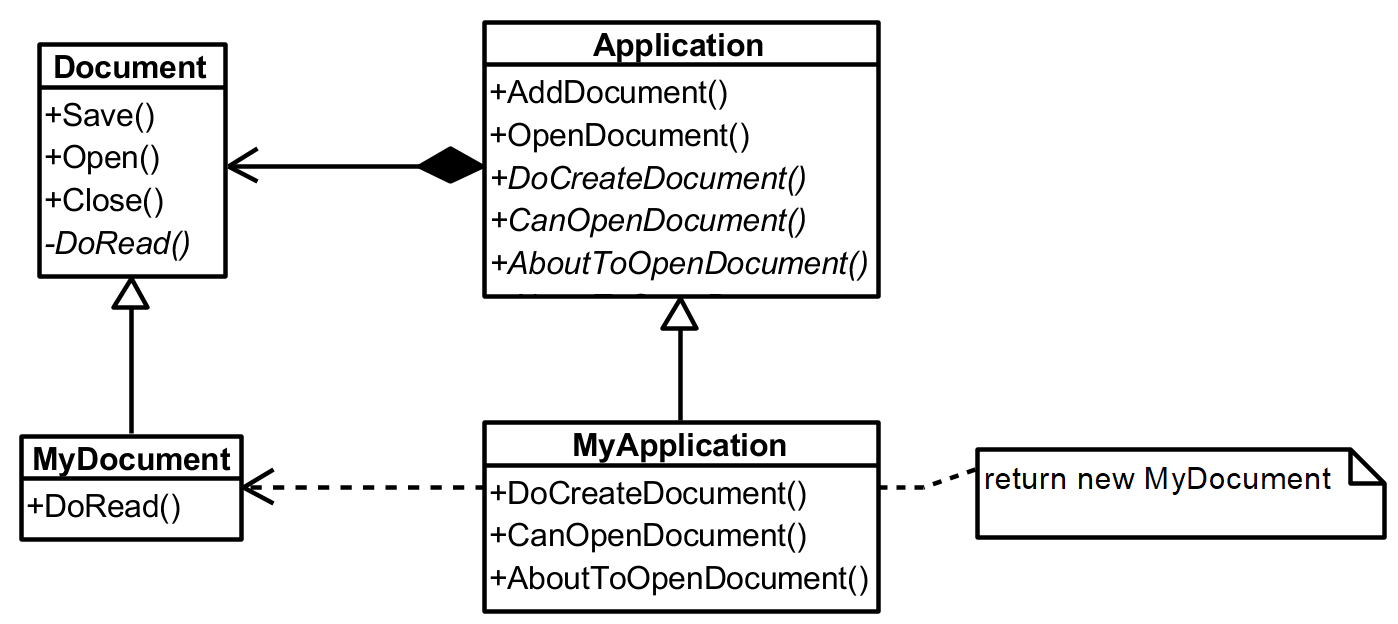
\includegraphics[width=0.8\textwidth]{templateMethodMotivation.png}
\end{center}

Тут операция добавления документа может использовать либо создание, либо открытие документа, и открытие документа состоит из нескольких этапов. Всё это описано в базовом классе, но что конкретно делать --- задаётся в потомках, которые не могут поменять общую схему работы, но могут в заранее фиксированных точках расширения определить свою функциональность. Некоторые методы предка могут иметь реализацию по умолчанию (как правило, пустую), что даёт потомкам расширить функциональность предка при необходимости, но не обязывает их это делать (как, например, в AboutToOpenDocument()). В коде это может выглядеть вот так:

\begin{minted}{cpp}
void Application::OpenDocument(const char* name) {
    if (!CanOpenDocument(name)) {
        return;
    }

    Document* doc = DoCreateDocument();
    
    if (doc) {
        _docs->AddDocument(doc);
        AboutToOpenDocument(doc);
        doc->Open();
        doc->DoRead();
    }
}
\end{minted}

DoCreateDocument(), к слову, --- это самый настоящий фабричный метод, играющий роль одной из элементарных операций шаблонного метода. Application::OpenDocument, кстати, и есть шаблонный метод.

\subsection{Шаблонный метод (Template method), общая структура}

Это обобщается до вот такой схемы:

\begin{center}
    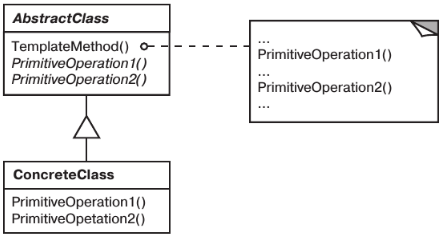
\includegraphics[width=0.6\textwidth]{templateMethod.png}
    \attribution{Э. Гамма и др., Приемы объектно-ориентированного проектирования}
\end{center}

AbstractClass определяет невиртуальный (как правило) TemplateMethod(), в котором фиксируется общий для всех потомков алгоритм, описанный в терминах абстрактных операций PrimitiveOperation1(), PrimitiveOperation2() и т.д. От абстрактного класса наследуются разные ConcreteClass, которые переопределяют примитивные операции. Поскольку алгоритм может быть довольно сложным, а примитивные операции довольно простыми, это позволяет легко переиспользовать алгоритм, облегчая создание новых ConcreteClass-ов и избегая копипаста.

\subsection{Детали реализации}

В плане реализации всё довольно просто, но надо принять решение, будут примитивные операции виртуальными или чисто виртуальными (или абстрактными, в зависимости от принятой в языке терминологии --- это суть одно и то же). Виртуальные имеют реализацию по умолчанию (часто пустую), что позволяет потомкам их не переопределять. Но потомок может \emph{забыть} их переопределить, что в случае чисто виртуальных операций не даст сделать компилятор. Так что чисто виртуальными следует делать те методы, которые обязательно надо переопределить (или хотя бы обязательно задуматься об этом), просто виртуальными --- те, без переопределения которых вполне можно обойтись.

В любом случае примитивные операции стоит делать protected, или, если язык позволяет, private (в C++ можно переопределять private-виртуальные методы предка, например). И, естественно, виртуальными, тогда как сам шаблонный метод, как правило, невиртуальный. Почему <<как правило>> --- для большей гибкости можно дать потомкам возможность при крайней нужде переопределить весь шаблонный метод целиком. Так, например, делают некоторые оконные библиотеки --- в Windows Forms есть конкретные методы наподобие OnPaint, которые можно перепределить в потомках, а есть виртуальный метод WndProc, который по умолчанию диспетчеризует сигналы операционной системы, как раз и вызывая всякие OnPaint, но если \emph{очень надо}, его можно переопределить по-своему (на практике автора этого ни разу не встречалось, впрочем). В общем случае это плохая идея, потому что она позволяет решить одну проблему двумя способами, что заставляет прикладного программиста задуматься (что уже плохо) и оставляет возможность сделать неправильно. Хорошая библиотека должна навязывать один способ решения задачи, либо делать альтернативы очень трудоёмкими, чтобы ими пользовались только те, кто знает, что делает.

Ещё стоит выбрать и использовать повсеместно единый стиль именования примитивных операций, например, называть их с префиксом <<Do>> (как в книжке рекомендуют) или с <<On>>, <<Handle>> и т.д. (как часто бывает в оконных библиотеках). Это позволяет быстро отличить методы, участвующие в паттерне <<Шаблонный метод>>, от других. Ну и, конечно, чем таких методов меньше (по крайней мере, чисто виртуальных), тем лучше --- иначе клиентам будет сложно понять, что именно им надо переопределить и зачем.

\section{Паттерн <<Посредник>>}

\subsection{Мотивирующий пример}

Допустим, мы хотим сделать окно настроек, позволяющее выбрать шрифт для нашего текстового редактора. Окно состоит из превью шрифта, выбиралки гарнитуры шрифта, вариантов начертания и размеров:

\begin{center}
    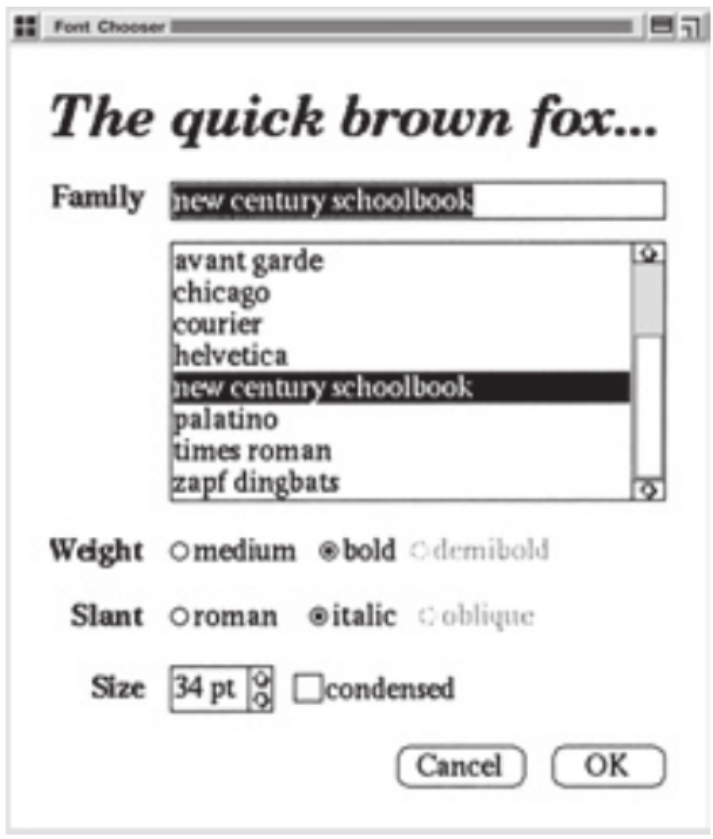
\includegraphics[width=0.4\textwidth]{mediatorMotivation.png}
    \attribution{Э. Гамма и др., Приемы объектно-ориентированного проектирования}
\end{center}

Сверстать такую форму несложно, однако мы хотим, чтобы при изменении параметров менялось и всё остальное. Превью зависит от всех параметров вообще, для некоторых гарнитур недоступны (видимо) некоторые варианты начертания, поле поиска гарнитуры должно обновляться при выборе гарнитуры из списка и наоборот. В общем, получается, что если одно поле изменилось, надо сказать об этом всем. Делать это каждому элементу управления, просто последовательно вызывая методы всех остальных элементов управления, плохая идея --- все должны знать про всех, и переиспользовать компоненты будет гораздо сложнее, поскольку окажется, что они способны работать только если есть все остальные.

Решение --- сделать отдельный объект, который будет отвечать за коммуникации между объектами. Тогда все остальные должны будут знать только про него, и отправлять нотификации об изменениях только ему. Он же, в свою очередь, рассылает нотификации всем остальным участникам взаимодействия:

\begin{center}
    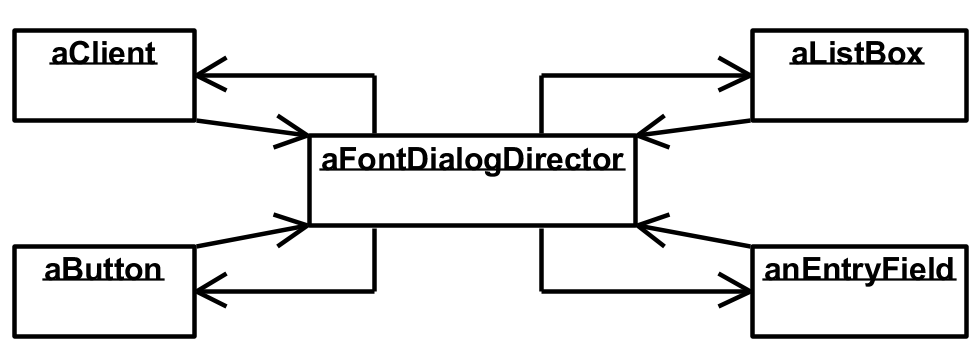
\includegraphics[width=0.7\textwidth]{mediatorObjectsDiagram.png}
\end{center}

Например, вот так может выглядеть пересылка сообщений об изменениях во время выполнения:

\begin{center}
    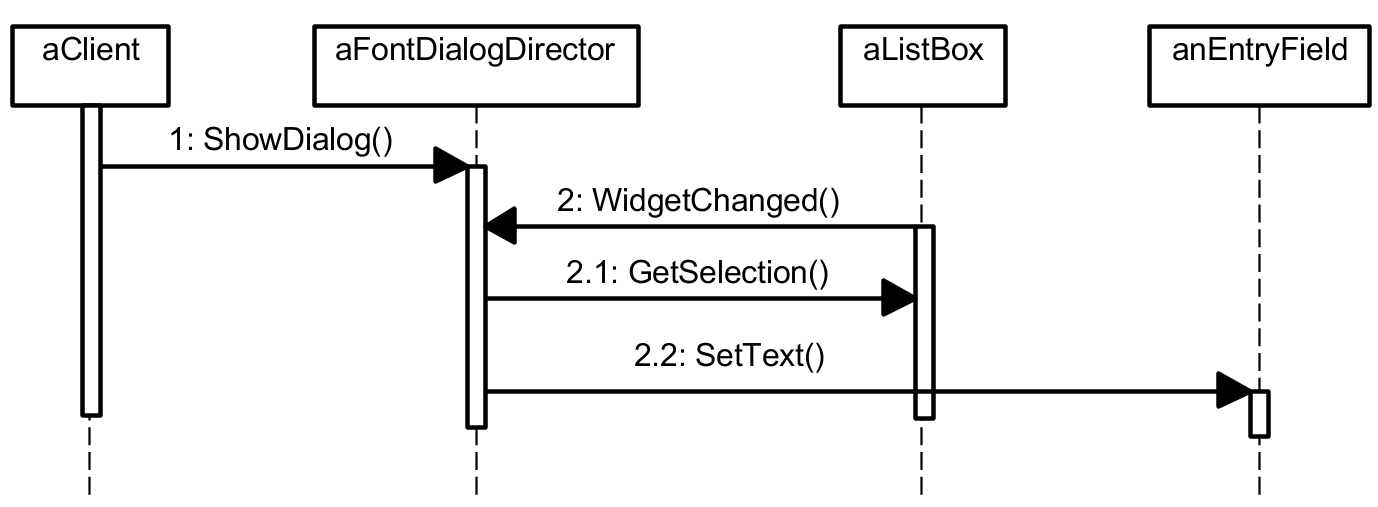
\includegraphics[width=0.9\textwidth]{mediatorSequence.png}
\end{center}

aFontDialogDirector (тот самый медиатор) инициализирует всю форму, сообщает о себе всем элементам управления, и, когда у них что-то происходит, запрашивает у них дополнительную информацию, и рассылает её всем, кому она интересна (причём, в данном примере медиатор сам знает, кому что рассылать). Структурно эта конструкция выглядит вот так:

\begin{center}
    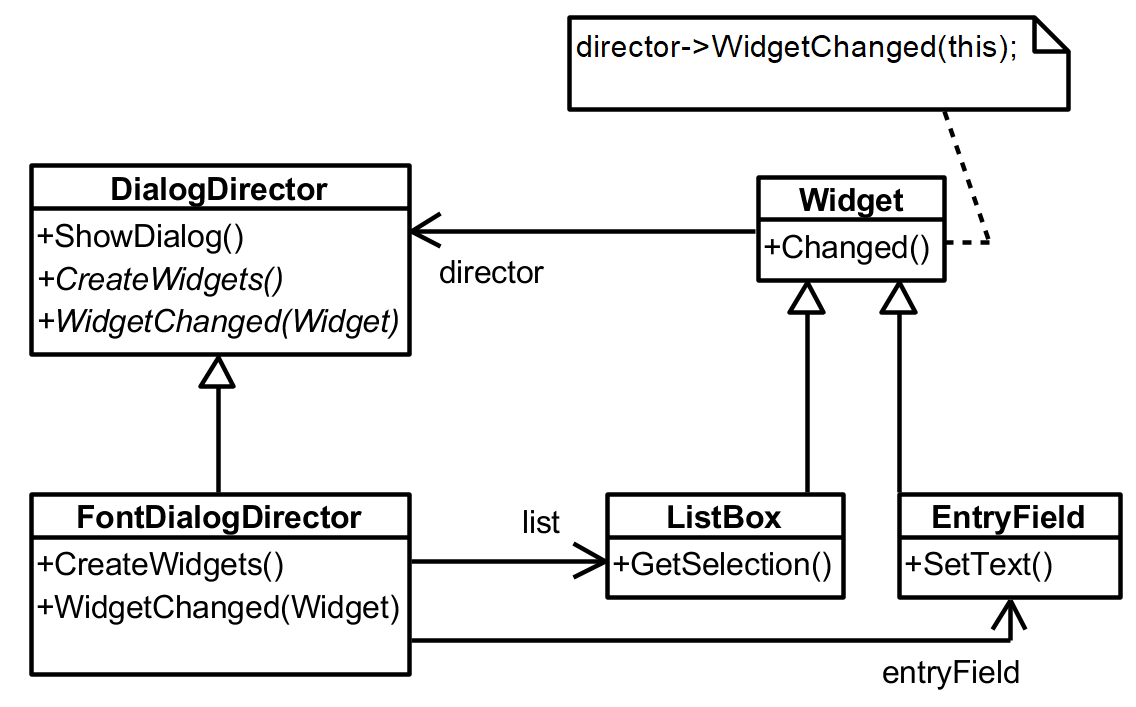
\includegraphics[width=0.7\textwidth]{mediatorStaticStructure.png}
\end{center}

Есть некоторый абстрактный класс DialogDirector, про который знают все Widget-ы (на самом деле, можно было обойтись конкретным FontDialogDirector-ом, но Архитектура!). FontDialogDirector знает про конкретные Widget-ы и умеет с ними общаться. Когда какой-то Widget говорит, что он изменился, FontDialogDirector понимает, какой именно изменился и что в нём поменялось, и сообщает остальным (только тем, кому это интересно).

\subsection{Посредник (Mediator), общая структура}

Общая статическая структура паттерна практически не отличается от мотивирующего примера:

\begin{center}
    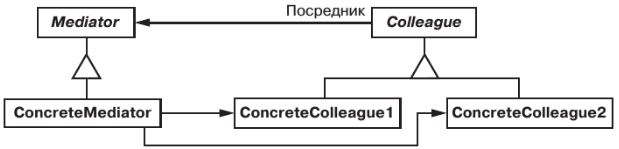
\includegraphics[width=0.8\textwidth]{mediatorClasses.png}
\end{center}

Абстрактный медиатор сам ни про кого не знает, но про него знают коллеги. Конкретный медиатор уже знает про всех коллег и может их нотифицировать. Абстрактный медиатор, кстати, чаще всего не нужен и его не реализуют --- коллеги общаются напрямую с конкретным медиатором. Во время выполнения структура объектов может выглядеть вот так:

\begin{center}
    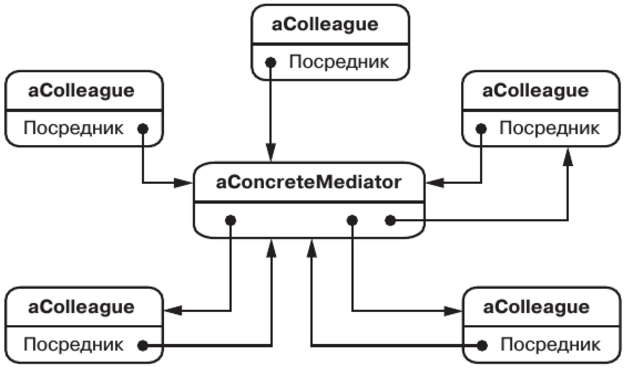
\includegraphics[width=0.7\textwidth]{mediatorObjects.png}
\end{center}

\subsection{Детали реализации}

С точки зрения реализации единственное по сути решение, которое надо принять --- это в какую сторону и как идёт обмен событиями. 

\begin{itemize}
    \item Можно использовать паттерн <<Наблюдатель>>: коллеги предоставляют события, на которые можно подписаться, медиатор подписывается на них и нотифицирует других коллег напрямую. Плюс такого подхода в том, что коллегам не надо знать про медиатора, что обычно хорошо, поскольку коллеги тогда могут быть стандартными библиотечными классами.
    \item Может быть и наоборот --- медиатор предоставляет событие <<что-то произошло>> или даже набор событий, на которые могут подписываться те коллеги, которым они интересны. Когда в коллеге что-то произошло, он вызывает медиатор напрямую, а медиатор уже распространяет сообщение о событии всем, кто на него подписался. При таком подходе каждому коллеге надо знать про медиатора, но самому медиатору зато не надо знать про коллег, и уже он может быть библиотечным классом. Кроме того, коллеги при такой схеме сами решают, на что подписаться и что посылать, так что проще управлять потоками событий (легко добавить нового коллегу в уже существующую систему, например). Такой подход используется в архитектурах с шиной событий и при применении очередей сообщений.
\end{itemize}

Итого, паттерн <<Медиатор>> полностью убирает ненужные связи между классами-коллегами, что способствует их переиспользованию (вплоть до использования библиотечных классов). Это способствует и упрощению взаимодействия между объектами, вместо квадратичной зависимости возможных связей от числа коллег получаем линейную. Кроме того, что важно при проектировании архитектуры системы в целом, медиатор абстрагирует и стандартизует общение между объектами.

Однако у паттерна есть важный недостаток, о котором надо всегда помнить при реализации --- это то место, которое знает про все (или очень многие) взаимодействия в системе. Что само по себе неплохо, но возникает соблазн сделать там содержательную логику диспетчеризации сообщений, затем конвертации из формата в формат, затем некоторую предварительную обработку перед доставкой коллегам, и вот --- мы получаем гигантский несопровождаемый God Object. Так делать ни в коем случае нельзя, медиатор должен заниматься только и исключительно организацией общения между коллегами, никакой бизнес-логики в нём быть не должно.

\section{Паттерн <<Команда>>}

\subsection{Мотивирующий пример}

Положим, у нас всё ещё есть текстовый редактор, над которым мы как бы работаем на протяжении всех лекций про паттерны. Теперь мы хотим сделать пользовательский интерфейс с командами, выполняющими всякие действия типа сохранения и загрузки файла, смены параметров шрифта и т.п. Причём, как и у всех приличных текстовых редакторов, у нас есть палитра инструментов, основное меню приложения, горячие клавиши --- и это на самом деле несколько способов вызвать одно и то же действие. Захардкодить в каждом пункте меню, что по его активации вызывается соответствующий метод бизнес-логики кажется плохой идеей --- получится, что элементы управления должны будут знать о классах бизнес-логики. Окей, мы можем применить паттерн <<Наблюдатель>> подписывать объект бизнес-логики на события от элементов управления, и это будет уже лучше, но тут мы вспомним, что надо ведь ещё поддержать undo/redo, и делать это в самой бизнес-логике нам бы очень не хотелось...

Решение --- обернём действие в объект: 

\begin{center}
    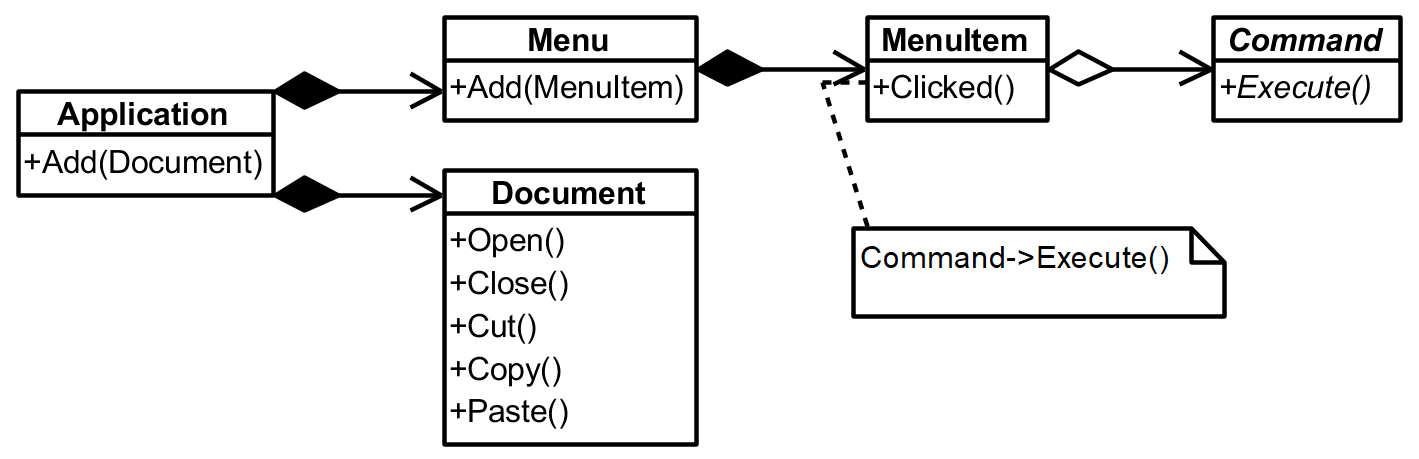
\includegraphics[width=0.9\textwidth]{commandExample.png}
\end{center}

Теперь сама команда --- это метод Execute() класса Command, и только он знает про бизнес-логику, которая реально исполняет команду (в данном примере она размещена в классе Document). Мы можем теперь создать объект Command и отдать его в главное меню, кнопке на палитре инструментов, менеджеру хоткеев и т.п., один и тот же объект, который исполняет одно действие. Таким образом, никто из потенциальных инициаторов команды не будет знать про то, что она делает (они видят только по сути интерфейс с одним методом). Это позволит легко менять команды разным элементам управления, и сделать их полностью независимыми от бизнес-логики. При этом команда может хранить в себе состояние, нужное для отмены операций.

Например, команда вставки:

\begin{center}
    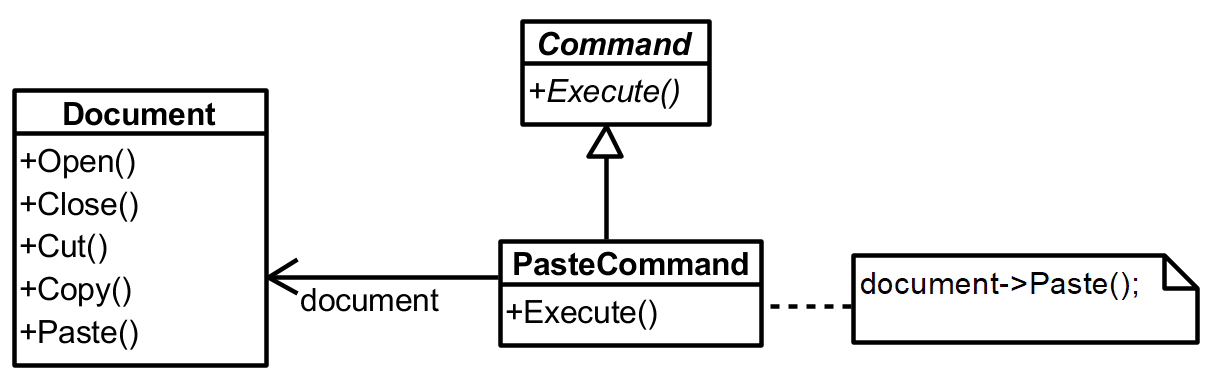
\includegraphics[width=0.8\textwidth]{pasteCommand.png}
\end{center}

PasteCommand реализует интерфейс Command очень простым образом --- она просто вызывает метод Paste() у класса с бизнес-логикой и больше ничего интересного не делает.

Или команда открытия документа:

\begin{center}
    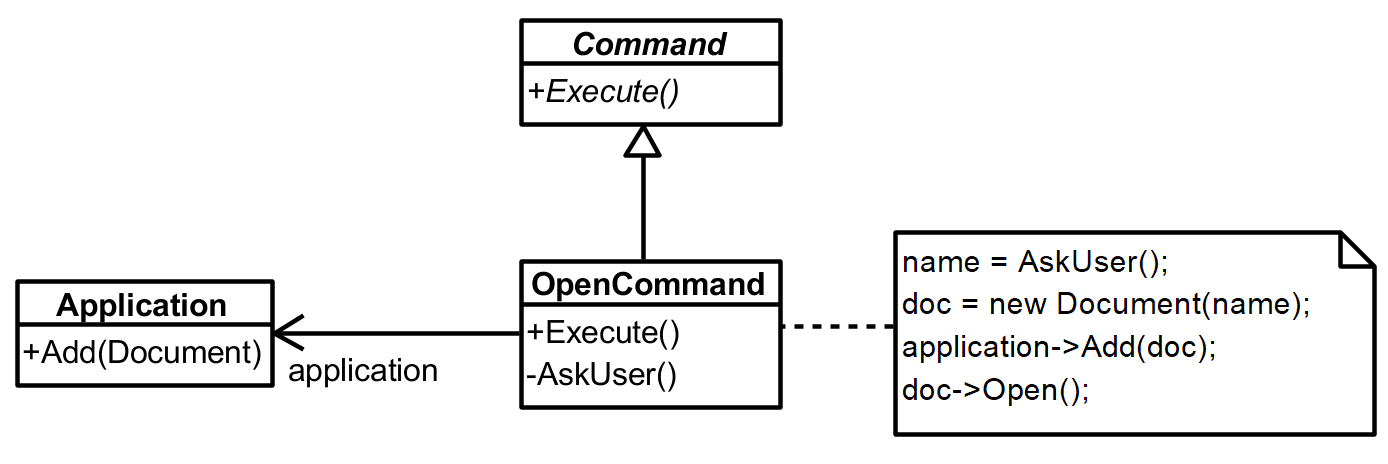
\includegraphics[width=0.8\textwidth]{openDocumentCommand.png}
\end{center}

Она уже сама содержит в себе логику взаимодействия с пользователем: сначала запрашивает у пользователя имя файла, потом создаёт документ, потом регистрирует его в приложении и открывает. Обратите внимание, команда, хоть и содержит нетривиальную логику, не реализует бизнес-логику работы с документами, она лишь взаимодействует с пользователем и <<оркестрирует>> основные классы системы.

А ещё команда может быть составной:

\begin{center}
    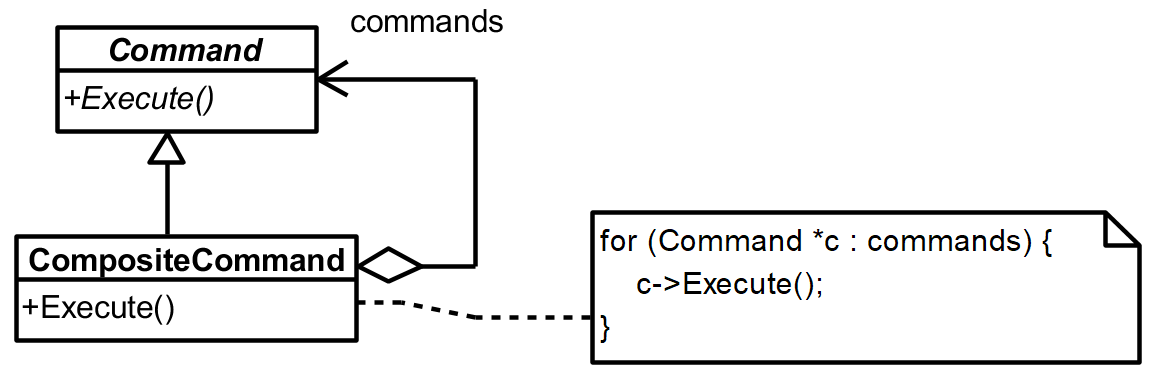
\includegraphics[width=0.7\textwidth]{compositeCommand.png}
\end{center}

Это полезно, когда один инициатор действия должен инициировать сразу несколько действий. Это позволяет легко поддержать макросы, но также полезно и для обычных команд: например, по нажатию на Enter в большинстве сред разработки выполняется переход на новую сроку и вставка отступа. В некоторых средах, если последовательно отменить эти действия, видно, что одно нажатие на Enter на самом деле спровоцировало два отдельных действия, с независимой отменой.

\subsection{Команда (Command), общая структура}

Идеи выше обобщаются до паттерна <<Команда>> с довольно нетривиальной структурой:

\begin{center}
    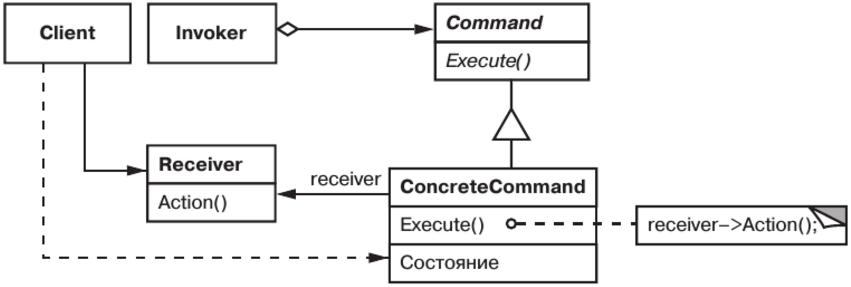
\includegraphics[width=0.8\textwidth]{command.png}
    \attribution{Э. Гамма и др., Приемы объектно-ориентированного проектирования}
\end{center}

Client --- это тот, кто пользуется всеми командами, как правило, это само приложение в целом (например, его функция main или аналог). Client создаёт классы, которые будут отвечать за бизнес-логику, стоящую за командами (класс Receiver), создаёт инициаторов действий (класс Invoker), создаёт конкретные команды, даёт им ссылки на их Receiver-ов и отдаёт Invoker-ам то, что получилось. Дальше, когда пользователь взаимодействует с приложением, он вызывает Invoker, тот вызывает виртуальный метод Execute() у Command, тот делает что-то полезное, вызывая Receiver:

\begin{center}
    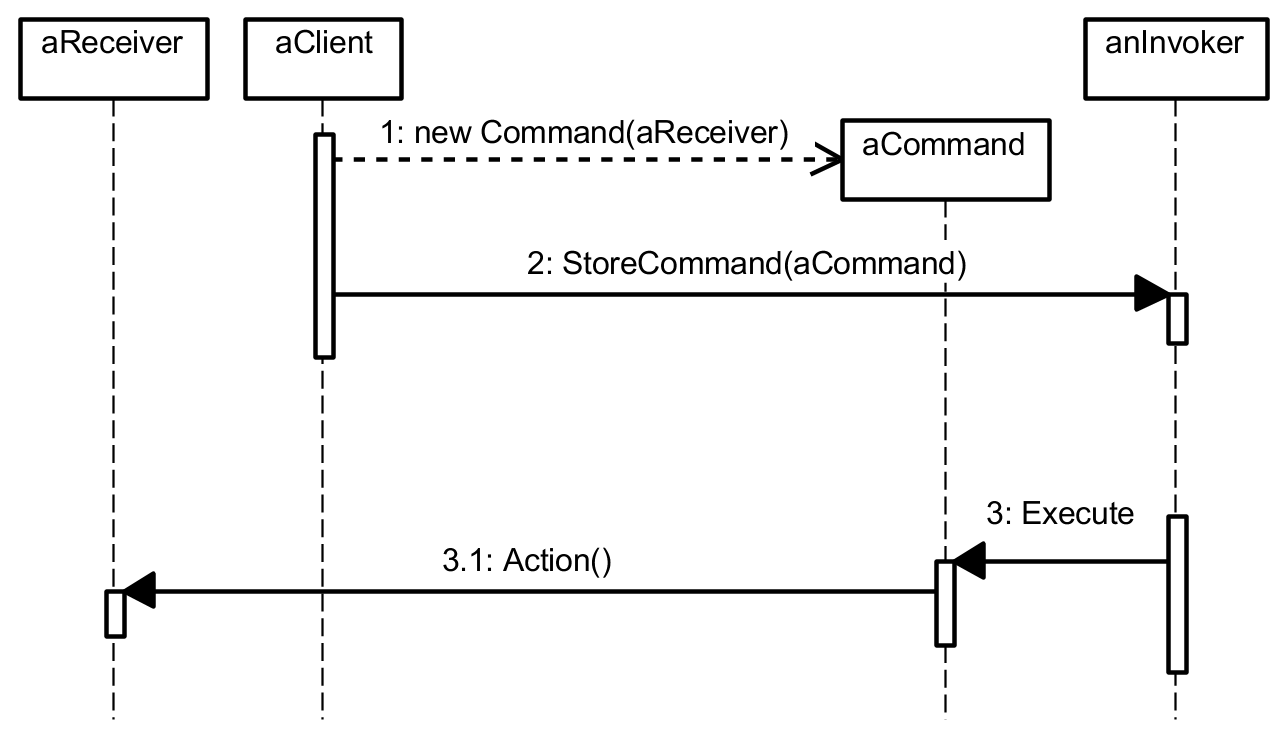
\includegraphics[width=0.8\textwidth]{commandSequence.png}
\end{center}

В нашем примере с редактором Client --- это Application, Receiver --- это Document, Invoker --- это MenuItem, а Command, кажется, очевидно кто.

Применяется этот паттерн, когда надо уметь работать с запросами как с объектами: хранить запросы, ставить в очередь на обработку, исполнять в произвольное время (ну, в большинстве случаев не в произвольное, а как будем готовы) и т.д. При этом команда --- это ещё и способ параметризовать объект исполняемым действием (то есть имеет <<встроенный>> паттерн <<Стратегия>>, Command же по сути Strategy для Invoker-а). Если немного расширить предложенную схему, легко поддержать отмену операций --- команда может хранить состояние, и если её не выкидывать после исполнения, может быть использована для возврата системы в вид, в котором она была до исполнения команды.

Архитектурно паттерн <<Команда>> тоже хорош, поскольку позволяет структурировать взаимодействие с пользователем. Если он последовательно применяется, то через команды проходит всё взаимодействие с пользователем, что позволяет иметь одно выделенное место в структуре системы, куда можно добавить логирование, валидацию и т.п. Кроме того, возможность собирать из простых команд составные (хоть полноценный паттерн <<Компоновщик>>) позволяет структурировать систему, собирая сколь угодно сложное взаимодействие с пользователем из элементарных операций.

В реальной жизни паттерн команда в том или ином виде есть в любой нормальной оконной библиотеке, так что непременно встретится на практике.

\subsection{Детали реализации}

С точки зрения реализации паттерн <<Команда>> предлагает на выбор массу архитектурных вариантов. Во-первых, насколько <<умной>> должна быть команда:

\begin{itemize}
    \item команда может вообще ничего не знать про логику работы приложения, да даже и про Receiver-а знать только то, что он есть и надо его дёрнуть, когда команду активируют;
    \item команда может выполнять всю полезную работу сама и никакой Receiver ей вообще не нужен;
    \item возможны и встречаются на практике также все промежуточные варианты.
\end{itemize}

<<Глупые>> команды хороши тем, что всю машинерию, связанную с командами, можно реализовать в библиотеке, и сами команды очень просты, выступая по сути исключительно методом связи Invoker-а и Receiver-а. Зато всю логику повторения и отмены операций, логирования и т.п. надо будет писать в Receiver-е, что для сложных систем может быть плохой идеей.

<<Умные>> команды могут быть идеальны, если всё приложение строится вокруг пользовательского интерфейса (например, штука для показа прогноза погоды или постов в Твиттере). Структурирование бизнес-логики по командам в этом случае может быть хорошей идеей с точки зрения архитектуры.

Однако команды, хоть и не привязаны к конкретным элементам управления, всё-таки слишком специфичны для приложения, поэтому переиспользовать их для другой задачи в рамках той же предметной области может быть проблематично. Поэтому часто используют не очень умные, но и не очень глупые команды --- команды, которые знают про логику взаимодействия с пользователем и сценарии использования конкретного приложения, но используют для своего исполнения объекты, моделирующие предметную область (они вообще ни о чём, кроме предметной области, знать не должны, поэтому великолепно переиспользуемы). В какой степени используют --- вопрос, на который приходится отвечать для каждой конкретной системы, так что можно сказать, что <<глупость-умность>> --- это шкала, причём шкала без дискретных значений.

Следующий архитектурный вопрос касается реализации отмены и повторения операций (Undo-Redo в англоязычной литературе). Делается это в целом довольно просто: заводятся два стека, Undo-стек и Redo-стек. Команде в дополнение к методу Execute() делают ещё метод Undo(). Когда команду исполняют впервые, вызывается её метод Execute() и команда кладётся на Undo-стек. Если пользователь хочет отменит операцию, с вершины Undo-стека снимается команда, вызывается её метод Undo() и команда перекладывается на Redo-стек. Если пользователь передумал отменять команду и хочет вернуть всё как было, команда снимается с вершины Redo-стека, снова вызывается её метод Execute() и команда кладётся на Undo-стек. Если исполняется какая-то новая команда (не с Undo- или Redo-стека), Redo-стек очищается. 

Обычно все эти стеки и механизм перекладывания команд туда-сюда реализуется в отдельном классе (обычно Controller), он же и исполняет команды --- то есть Invoker не вызывает на самом деле сам Execute(), он просто вызывает контроллер, отдавая ему активированную команду.

Собственно, архитектурный вопрос в том, как реализовать операцию Undo() в команде. Это опять зависит от конкретной задачи. Можно хранить в команде всё состояние системы целиком, а в Undo() просто возвращать систему в исходное состояние. Можно хранить дельту относительно предыдущего состояния и вычислять обратное преобразование, которое отменит команду (например, в текстовом редакторе команде добавления буквы в текст достаточно просто запомнить позицию добавленной буквы, чтобы в Undo() её удалить --- но помните, что при повторном вызове Execute() нам надо иметь возможность повторить команду, так что надо запомнить и позицию, и саму букву).

Выше говорилось, что, мол, есть команда, это один объект, который раздаётся разным Invoker-ам, а тут ещё, оказывается, он хранится в Undo- или Redo-стеке и запоминает состояние. А что будет, если одну и ту же команду активировали дважды? Да, это проблема, и если команда мутабельна (то есть правда хранит состояние), перед тем, как её исполнить в первый раз, надо её скопировать. Может помочь паттерн <<Прототип>>.

Также могут быть полезны искусственные команды --- то есть команды, которые не активируются ничем из пользовательского интерфейса, а добавляются в контроллер другими классами системы. Это при неаккуратной реализации может удивить пользователя (когда он сможет отменить то, чего сам никогда не делал), но это решается наличием в команде одного булевого флага, что она искусственная. Также применяются и композитные команды, которые позволяют одно действие из пользовательского интерфейса исполнить с помощью нескольких элементарных команд. Откатывать лучше всю композитную команду целиком, поэтому желательно класть на стек именно её, а не её подчинённые команды.

Паттерн <<Команда>> в плане отката операций хорошо комбинируется с паттерном <<Хранитель>>. <<Хранитель>> может сделать слепок состояния системы (или части состояния, необходимой для восстановления), отдать его команде, а потом, при отмене команды, восстановить состояние системы из слепка. Команда в этом случае выступает в роли Caretaker-а из паттерна <<Хранитель>> (про который чуть позже).

Вот пример <<глупой>> команды из реального мира, оконной библиотеки для C++ со звучным названием Qt\footnote{в C++ много чего называется совершенно непроизносимо, хотя конкретно Qt читается как <<кьют>>, созвучно английскому <<cute>>, <<милый>> --- или \emph{они} хотят заставить нас в это поверить.}:

\begin{minted}{c++}
const QIcon openIcon = QIcon(":/images/open.png");
QAction *openAct = new QAction(openIcon, tr("&Open..."), this);

openAct->setShortcuts(QKeySequence::Open);
openAct->setStatusTip(tr("Open an existing file"));

connect(openAct, &QAction::triggered, this, &MainWindow::open);

fileMenu->addAction(openAct);
fileToolBar->addAction(openAct);
\end{minted}

Команда тут --- это класс QAction. Ей при создании выдают иконку, текст названия команды (используется функция tr, возвращающая перевод (<<translation>>) строки для текущей локали), задаётся горячая клавиша (привязанная к константе, соответствующей Ctrl-O или чему-то такому в зависимости от операционной системы), всплывающая подсказка. Дальше с помощью функции connect и Qt-шной магии (весьма продвинутой, к слову --- в Qt есть собственный препроцессор и кодогенератор, запускающийся до основной компиляции) событие triggered команды связывается с обработчиком open класса MainWindow. MainWindow в данном случае выступает в роли Receiver-а из паттерна. Дальше команда отдаётся основному меню приложения и панели инструментов, которые используют иконку и текст команды, чтобы отобразить их на кнопке и в пункте меню соответственно. Теперь, когда пользователь активирует команду (например, нажав хоткей или кликнув на кнопку на панели инструментов), команда активирует событие triggered, что приведёт к вызову метода open у объекта MainWindow. 

Тут команда вообще просто библиотечный класс и всю работу делает Receiver. Пользоваться такой командой очень удобно при разработке пользовательских интерфейсов, однако для организации обработки запросов глубоко внутри приложения такая реализация не годится (иконка нужна, например). Автору пришлось писать свой аналог вручную, чтобы использовать команды для обработки заданий в глубине приложения.

\section{Паттерн <<Цепочка ответственности>>}

\subsection{Мотивирующий пример}

Положим, у нас снова есть наш текстовый редактор, хотя подойдёт и любое приложение с оконным интерфейсом. И положим, мы хотим сделать контекстную справку --- в Windows, например, некоторые окна имеют справа вверху кнопку с вопросиком, при нажатии на которую и последующем нажатии на элемент управления появляется всплывающая подсказка, описывающая, что этот элемент управления делает. Мы хотим сделать архитектурно удобную систему, которая предоставляла бы контекстную справку по клику мышью, так, что если для данного элемента контекстная справка недоступна, показывается контекстная справка элемента, в котором он содержится. А если и для объемлющего элемента контекстной справки нет, то спрашиваем у элемента, в котором содержится он, и т.д.:

\begin{center}
    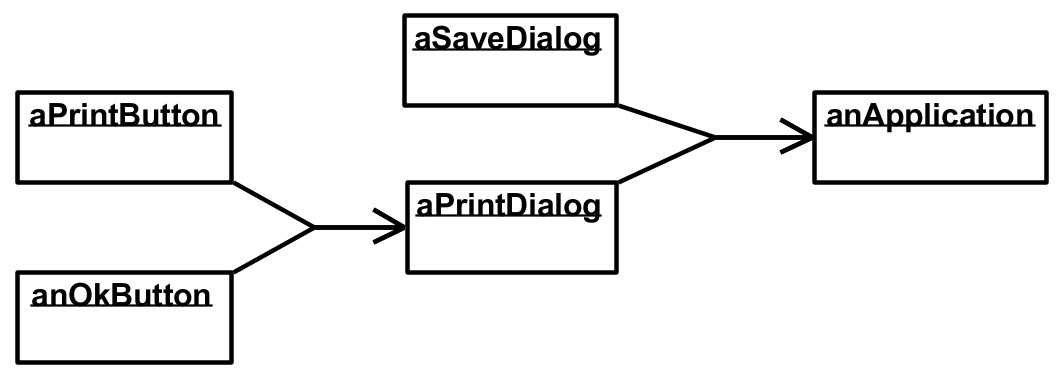
\includegraphics[width=0.6\textwidth]{chainOfResponsibilityExample.png}
\end{center}

Если так ни у кого контекстной справки и не нашлось, никто ничего и не покажет, что в данном случае вполне ок (ну не сделали справку пока, что ж делать). На диаграмме классов это могло бы выглядеть как-то так:

\begin{center}
    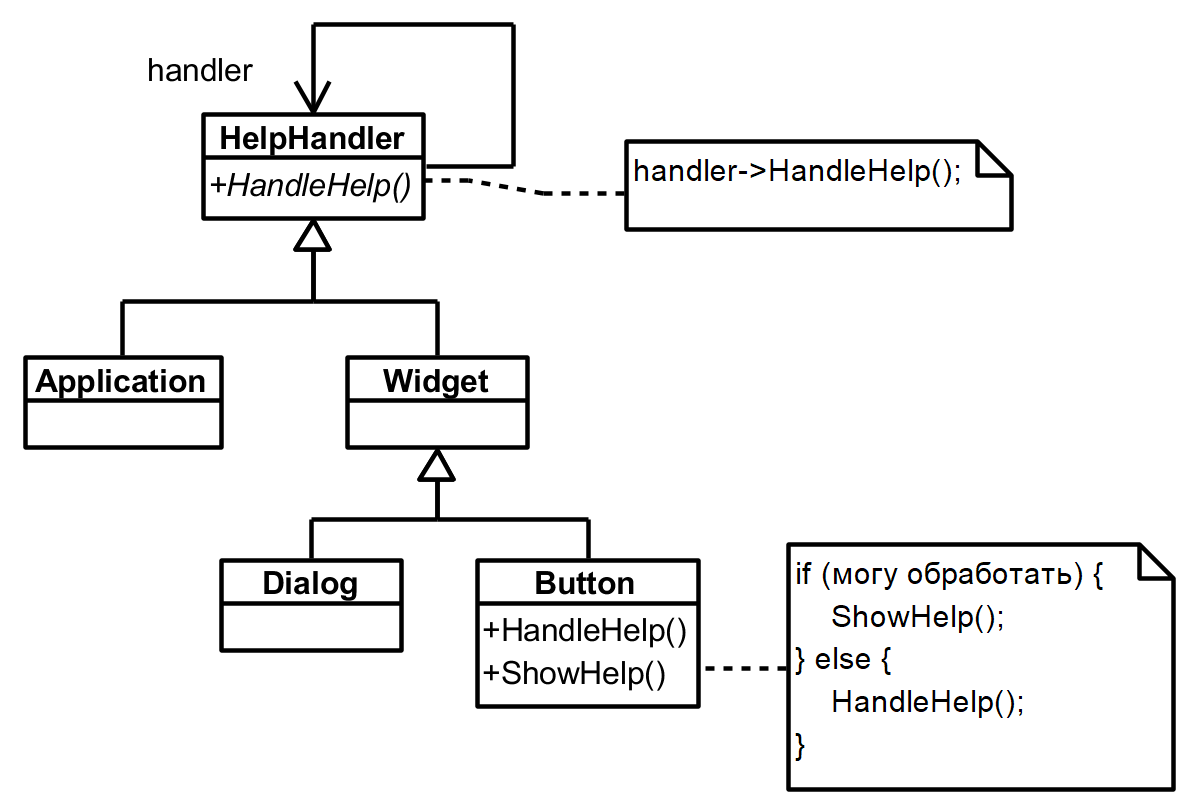
\includegraphics[width=0.7\textwidth]{chainOfResponsibilityExampleClasses.png}
\end{center}

Базовый класс <<Обрабатывалка запросов помощи>> содержит ссылку на того, кому надо передать запрос дальше, если он не обработал, и реализацию по умолчанию обработчика --- которая просто передаёт запрос дальше по цепочке. От базового класса наследуются конкретные классы, например, Button, где HandleHelp() переопределяется так, что если мы можем обработать запрос, обрабатываем, если нет, передаём дальше (вызовом метода предка, чтобы не вручную).

\subsection{Цепочка ответственности (Chain of Responsibility), общая структура}

Обобщается эта идея до вот такой структуры:

\begin{center}
    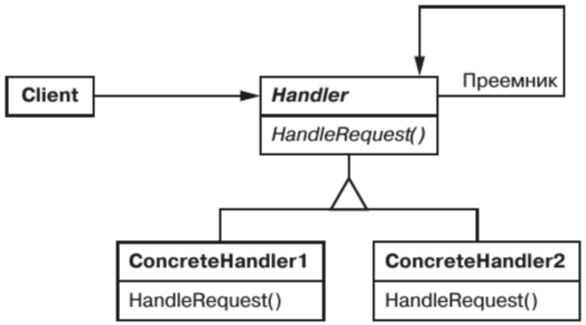
\includegraphics[width=0.6\textwidth]{chainOfResponsibility.png}
    \attribution{Э. Гамма и др., Приемы объектно-ориентированного проектирования}
\end{center}

Всё как в примере, есть базовый класс, который организует цепочку, и имеет метод по умолчанию, который просто передаёт запрос дальше. От него наследуются конкретные классы, которые переопределяют HandleRequest(), и если не могут обработать запрос, вызывают метод предка.

Используется этот паттерн, когда есть более одного потенциального обработчика запроса и мы не знаем (или не хотим знать), какой именно обработчик должен обработать запрос. Такое может происходить, когда обработчики могут добавляться в цепочку или удаляться из неё динамически, в том числе подгружаясь из плагинов. Ещё, в классическом паттерне предполагается, что если запрос обработан, он дальше не распространяется --- но иногда полезно, чтобы запрос двигался по цепочке дальше и, возможно, был обработан несколькими объектами сразу.

<<Цепочка ответственности>> позволяет уменьшить связность системы, разрывая жёсткую связь между отправителем запроса и его получателем, и даёт возможность реконфигурировать обработку запроса динамически, что повышает гибкость. Однако за это приходится платить --- паттерн не гарантирует, что запрос вообще в принципе будет обработан, и отправитель может даже не узнать, что его запрос пропал.

\subsection{Детали реализации}

Дьявол, как обычно, кроется в деталях. Первое, что надо учитывать --- это что, как правило, цепочка уже есть: в оконных библиотеках элементы управления и так образуют дерево, обработчики в системах обработки событий и так связаны в список, и т.д. С большой вероятностью ссылка <<Преемник>> у вас и так уже есть и её делать не надо.

Если возможных запросов несколько, их надо как-то различать. Для этого можно сделать несколько методов, <<Handle-то()>>, <<Handle-сё()>>, но при добавлении нового вида запросов придётся менять вообще всю иерархию обработчиков. Чаще делают хитрее --- запрос представляется в виде объекта, и есть один метод <<Handle(BaseRequest request)>>. BaseRequest в таком случае --- это просто абстракция запроса, и у него есть наследники, например, ConcreteRequest1, ConcreteRequest2 и т.д., у каждого могут быть свои поля, в которых передаются данные, необходимые для обработки запроса. Теперь ConcreteHandler-ы могут делать проверку типа и динамический каст, и если видят, что такие запросы обрабатывать умеют, обрабатывают, а если нет, просто передают дальше. Теперь добавление нового вида запроса --- это просто добавление нового наследника BaseRequest, код существующих обрабобтчиков менять не надо. Например, в .NET есть класс EventArgs, который никаких данных не содержит, у него есть наследники MouseEventArgs с координатами клика, KeyEventArgs с кодом нажатой клавиши и т.д. В обработчик событий элемента управения передаётся EventArgs, он сам смотрит на него и в зависимости от типа времени выполнения диспетчеризует. Так что если добавить новый тип события или уточнить существующий (например, ввести KeyPressEventArgs, наследующийся от KeyEventArgs\footnote{В реальной жизни оба эти класса наследуются прямо от EventArgs, но для примера сойдёт.}), ничего не сломается.

Ещё два примера применения этого паттерна в реальной жизни: во-первых, распространение исключений можно считать <<Цепочкой ответственности>>. throw выступает в роли клиента, который шлёт запрос, блоки catch --- в роли обработчиков, которые, если знают, как обработать запрос, обрабатывают его, если нет --- выбрасывают исключение дальше по стеку вызовов. Как и в паттерне, никто не гарантирует, что исключение обязательно будет поймано, и если нет, программа аварийно заканчивает работу.

Вот второй пример, распространение событий в оконных библиотеках (в данном случае, Qt):

\begin{minted}{c++}
void MyCheckBox::mousePressEvent(QMouseEvent *event)
{
    if (event->button() == Qt::LeftButton) {
        // handle left mouse button here
    } else {
        // pass on other buttons to base class
        QCheckBox::mousePressEvent(event);
    }
}
\end{minted}

QMouseEvent event --- это тот самый объект-событие, про который говорилось выше. Он содержит в себе сведения о том, что произошло, в частности, какая кнопка была нажата. Если левая, то обрабатываем событие и на этом заканчиваем его распространение, если нет --- отдаём обработку базовому классу QCheckBox, который либо сам что-то сделает (почему нет, QCheckBox вполне может имет поведение по умолчанию при клике на него), либо отдаст контролу, в котором он содержится.

\section{Паттерн <<Состояние>>}

\subsection{Мотивирующий пример}

На сей раз положим, что нам внезапно надо реализовать сетевой стек операционной системы. У нас есть класс TcpConnection, с методами открытия, закрытия и подтверждения, и он может находиться в трёх состояниях: соединение установлено, ожидаем соединения, соединение закрыто. Рабоче-крестьянская реализация предполагает наличие переменной-состояния в TcpConnection, по которой в каждом методе делается switch --- и, например, если мы пытаемся вызвать Open() для уже открытого соединения, то ничего не делаем. Но, как мы знаем, если у нас много где разные действия выполняются в зависимости от значения какой-то переменной, то это code smell <<тэг типа>> и его можно заменить на иерархию наследования. Так получаем уже почти паттерн <<Состояние>>:

\begin{center}
    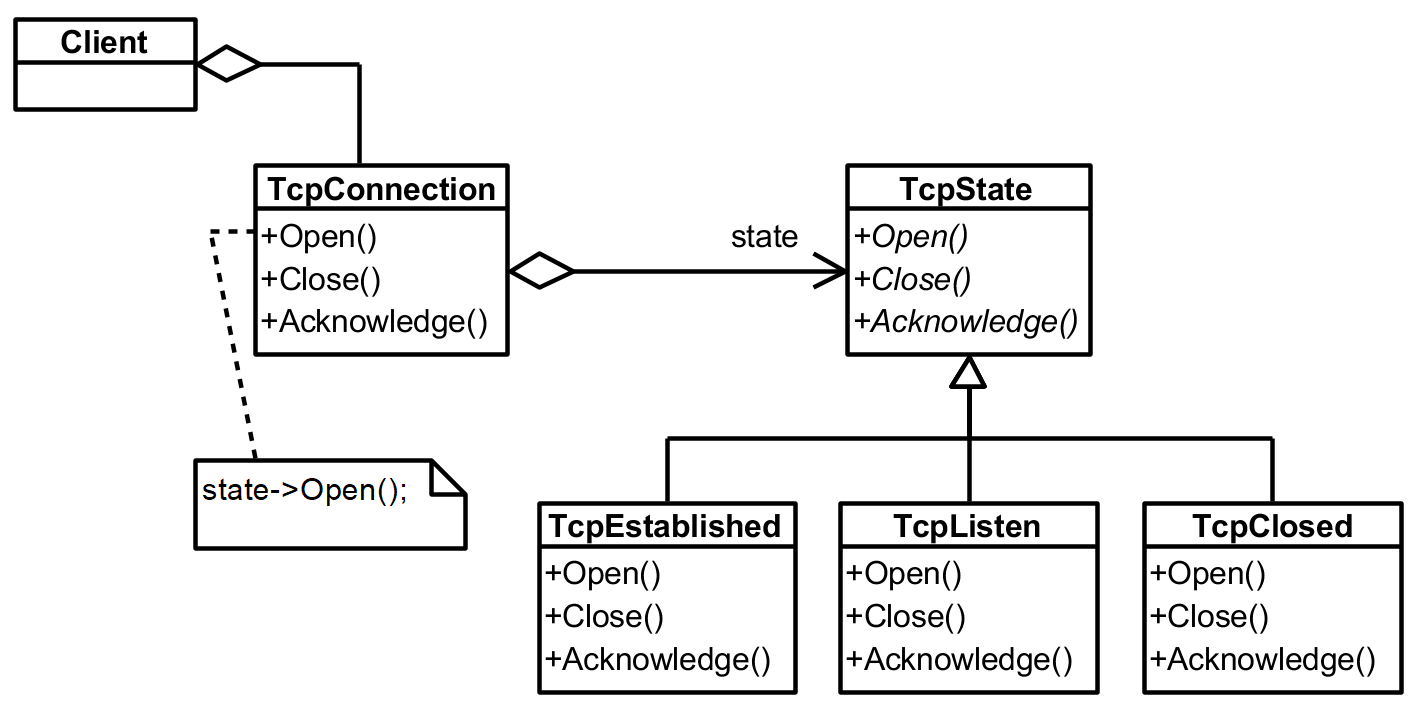
\includegraphics[width=0.75\textwidth]{stateExample.png}
\end{center}

Внешне это очень похоже на паттерн <<Стратегия>> --- есть контекст (TcpConnection), который делегирует свои основные действия объекту-состоянию (например, TcpEstablished), который их и выполняет. И в зависимости от того, в каком состоянии мы находимся, TcpConnection работает по-разному, причём переключение состояний незаметно для клиента --- он просто вызывае методы TcpConnection и не знает, что там происходит внутри. Важное отличие от <<Стратегии>> в том, что TcpConnection может переходить из состояния в состояние сам, и паттерн на самом деле определяет, как это реализуется, тогда как в <<Статегии>> требуется участие клиента для смены стратегии. То есть <<Состояние>> можно понимать как некоторую специализированную <<Стратегию>> плюс возможность автоматически переключать поведение.

\subsection{Состояние (State), общая структура}

Общая структура паттерна такова:

\begin{center}
    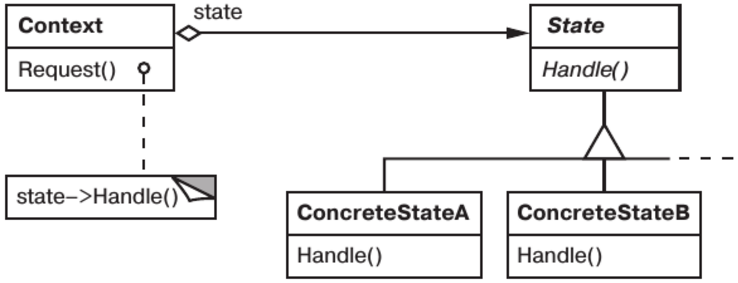
\includegraphics[width=0.6\textwidth]{state.png}
    \attribution{Э. Гамма и др., Приемы объектно-ориентированного проектирования}
\end{center}

Клиент пользуется объектом класса Context, который делегирует запрос одному из наследников класса (чаще интерфейса) State, при этом либо в Context, либо в наследниках State определяется механизм перехода из состояния в состояние. Таким образом, несмотря на то, что Context остаётся одним объектом, с точки зрения клиента всё выглядит так, будто он динамически меняет свой класс во время выполнения (как будто его методы виртуальные и у него меняется тип времени выполнения в зависимости от ситуации). Языки со строгой типизацией такого для обычных классов не позволяют, а паттерн <<Состояние>> позволяет добиться такой вот симуляции динамической типизации, что иногда бывает полезно.

Применяется этот паттерн тогда, когда поведение объекта зависит от его состояния, которое может меняться во время выполнения --- вот, например, сетевые подключения, или на самом деле все системы, выражающиеся в терминах конечных автоматов (а это большинство реактивных систем, начиная от дверного замка, заканчивая робототехническим комплексом или ИИ в компьютерных играх). Паттерн <<Состояние>> также идеален для реализации <<вручную>> конечных автоматов. Ну и в чисто прагматических целях минимизации switch, if-ов и т.п., особенно если класс явно хранит что-то, похожее на стостояние, паттерн может быть полезен.

Преимущества его применения (по сравнению с другими способами реализации конечных автоматов) в том, что действия в каждом состоянии инкапсулированы в отдельный класс, так что каждое состояние легко сопровождать, да и добавлять состояния несложно. И переходы между состояниями делаются явными, что упрощает дизайн автомата. Для применений, требующих скорости работы, однако, такой подход используется редко --- например, в лексических анализаторах скорее сгенерированнные таблицы переходов, они при аккуратной реализации работают в разы быстрее (что неудивительно, нет затрат на виртуальные вызовы и перенаправление запросов).

\subsection{Детали реализации}

Самое интересное при реализации паттерна --- это переходы между состояниями. Их можно делать в Context (то есть сам автомат управляет переходами) или в конкретных State (то есть каждое состояние знает, какое должно быть следующим при каком входе). Делают и так и так. Первый способ проще в плане управления состояниями (понятно, когда их создавать и удалять), и уддобен тем, что есть центральное место, которое реализует логику переходов. И, кстати, логика эта может быть реализована в виде таблицы переходов --- отображения текущего состояния и входного сигнала в следующее состояние. При таком подходе, правда, сложно реализовать действие при переходе, поэтому этот способ довольно ситуационный. Второй способ --- когда само состояние возвращает при вызове действия следующее состояние --- в этом плане более гибок, но тогда логика переходов размазана по нескольким классам и в ней легко запутаться.

Ещё возникает вопрос с созданием и удалением объектов-состояний. Часто состояний немного, так что нет ничего плохого в том, чтобы создать из раз и навсегда, хранить в Context и отдавать друг другу, чтобы они знали, куда переходить. Но бывают и большие автоматы (из миллионов состояний --- надеемся, что по логике почти одинаковых), для них, возможно, более правильно было бы создавать следующее состояние при переходе в него из текущего, и удалять текущее. Но делать это надо аккуратно, чтобы не удалить состояние до того, как оно создало следующее (ошибки типа delete this;, например, иногда встречаются в коде на C++).

Ещё состояния часто могут быть разделяемыми между несколькими автоматами, особенно если не содержат никаких данных. Паттерны <<Пул объектов>> или <<Приспособленец>> помогут управлять разделяемыми состояниями. С другой стороны, обычно овчинка выделки не стоит, но ситуации бывают разные (например, некоторые алгоритмы распознавания предполагают создание нового автомата на каждый входной символ, так что легко получить миллион автоматов из нескольких сотен состояний --- там этот приём может быть полезным).

\section{Паттерн <<Посетитель>>}

\subsection{Мотивирующий пример}

Для паттерна <<Посетитель>> в качестве мотивирующего примера возьмём самое частое его использование в реальной жизни --- написание компиляторов. Положим, у нас есть абстрактное синтаксическое дерево и мы хотим выполнять над ним разные операции, например, проверку типов, печать, кодогенерацию. Можно сделать как на рисунке:

\begin{center}
    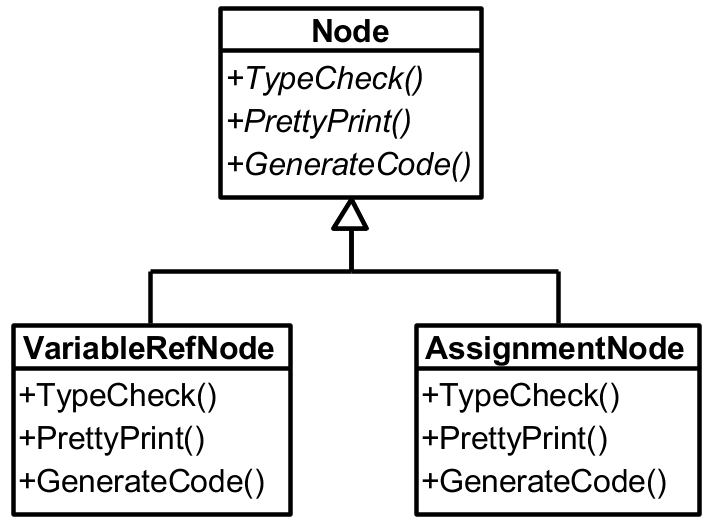
\includegraphics[width=0.45\textwidth]{visitorExample.png}
\end{center}

То есть завести базовый класс для всех узлов синтаксического дерева (и так обычно всегда и делают) и определить все операции в нём (а вот так обычно как раз не делают). Не делают так потому, что разных типов узлов в дереве обычно примерно стлько, сколько продукций в грамматике языка, то есть, для настоящих языков программирования, от нескольких десятков до нескольких сотен.  Реализовывать в каждом узле по N операций и обновлять всю иерархию наследования каждый раз, когда добавляется или изменяется какая-то операция --- слишком утомительно.

Решение этой проблемы --- как обычно, вынести операцию в отдельный класс, и дать ей воззможность применяться к разным видам узлов. Это и есть идея паттерна <<Посетитель>>. В узлах абстрактного синтаксического дерева определяется только одна операция, Accept, которая принимает абстрактный посетитель (обычно это интерфейс), в абстрактном посетителе объявлены методы, по одному для каждого класса узла, которые должны выполнять над этим узлом операцию. Операция реализуется в конкретных посетителях:

\begin{center}
    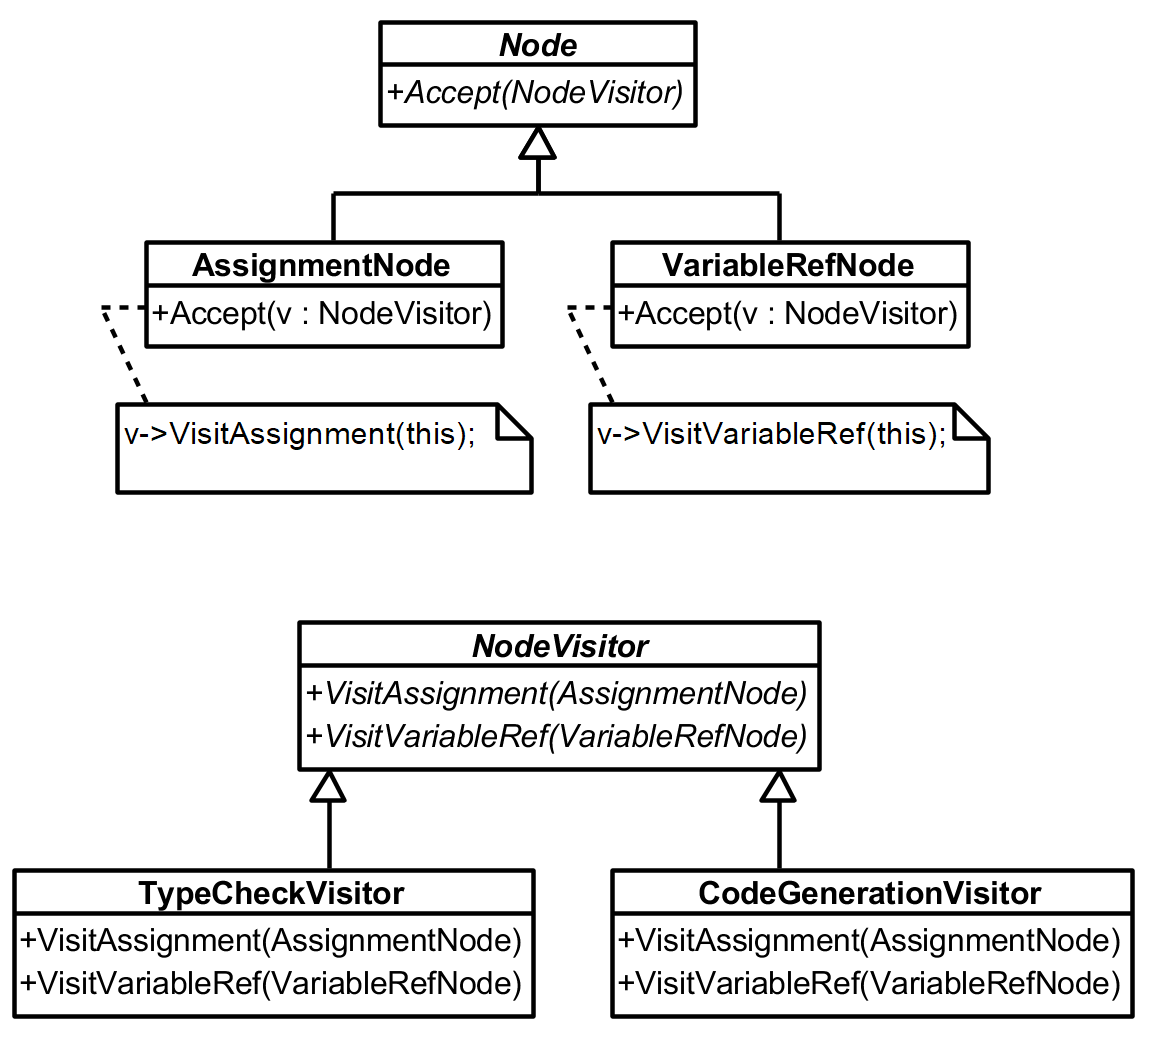
\includegraphics[width=0.65\textwidth]{visitorExampleSolution.png}
\end{center}

\subsection{Посетитель (Visitor), общая структура}

Эта идея обобщается до общей схемы паттерна:

\begin{center}
    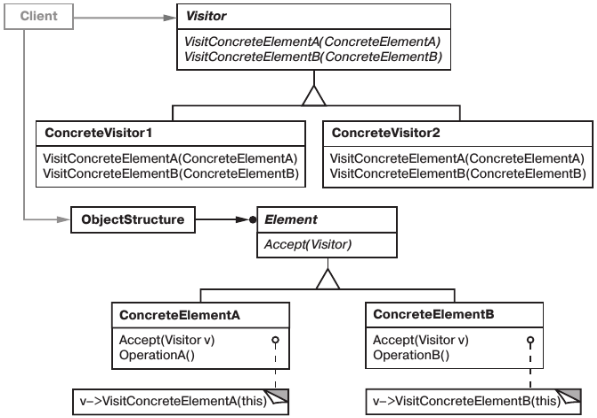
\includegraphics[width=0.9\textwidth]{visitor.png}
    \attribution{Э. Гамма и др., Приемы объектно-ориентированного проектирования}
\end{center}

Есть некая структура данных (ObjectStructure), которая состоит из элементов разных типов с общим базовым классом (если все элементы одного типа, это уже паттерн <<Итератор>>). Чтобы что-то с ней сделать, клиент создаёт конкретный Visitor и отдаёт его ObjectStructure, которая последовательно вызывает Accept для каждого элемента. А Accept ничего содержательного не делает, а просто вызывает соответствующий себе Visit у переданного Visitor-а. Во время выполнения это работает как-то так:

\begin{center}
    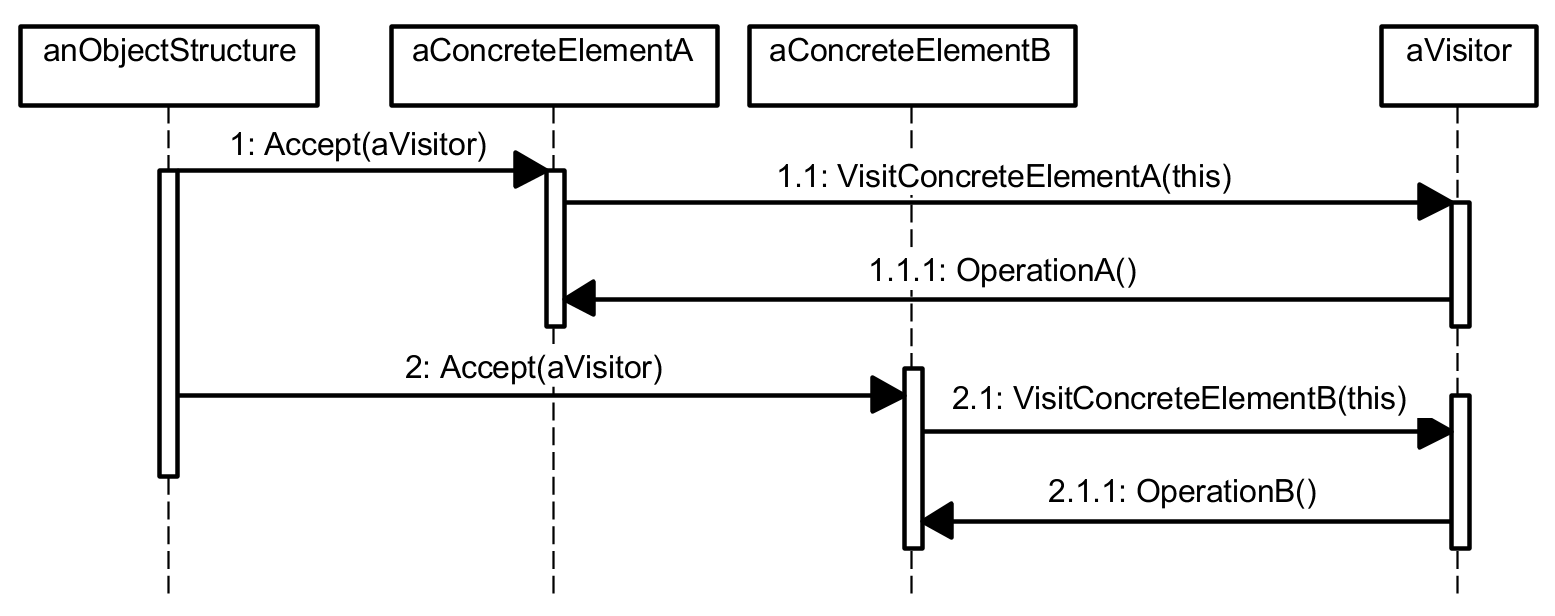
\includegraphics[width=0.8\textwidth]{doubleDispatching.png}
\end{center}

Такая схема называется <<двойная диспетчеризация>>, в противоположность одинарной диспетчеризации --- обычному виртуальному вызову. При вызове виртуального метода код, который надо исполнить, определяется типом времени выполнения объекта, от которого делается виртуальный вызов. При двойной диспетчеризации исполняемый код определяется типом двух объектов --- в нашем случае, элемента и посетителя. Сначала вызываем виртуальный метод Accept у элемента, попадаем в конкретный элемент, который взывает виртуальный метод Visit... у посетителя и попадает в конкретный посетитель и его метод для конкретного элемента.

\subsection{Детали реализации}

Есть два варианта реализации методов Visit() --- это VisitClassA(), VisitClassB(), или все методы Visitor-а можно назвать Visit() и использовать перегрузку. При вызове Visit() компилятор знает точный тип параметра, поэтому может понять, какую из перегрузок вызвать. Кажется, что перегруженный Visit() элегантнее, однако в книжках не рекомендуют так делать, потому что первый способ (когда у Visit в названии тип аргумента) более читаемый --- не только компилятор, но и человек сразу может понять, какой из методов вызывается.

Следующий важный момент --- кто управляет обходом. Описание выше выглядит так, будто коллекция принимает Visitor и сама управляет обходом, последовательно передавая Visitor своим элементам. Однако часто обходом управляют сами элементы коллекции, потому что только они знают, как попасть к своим сыновьям. Иногда обходом управляет сам Visitor --- это особенно полезно, когда обход зависит от результата посещения конкретного элемента (например, не надо идти в правый аргумент логического <<и>>, если левый false). В таком случае Visitor просит сыновей у переданного ему элемента и сам вызывает у них Accept(this).

При обходе Visitor вполне может накапливать в себе состояние, и даже строить преобразованную структуру данных (то есть Visitor можно использовать для реализации чего-то вроде функций map и fold, типичных для функциональных программ). Например, в компиляторах этот паттерн нередко используется для преобразования синтаксических деревьев.

Надо помнить, что у Visitor есть пара известных недостатков:
\begin{itemize}
    \item он несколько нарушает инкапсуляцию --- элементы коллекции должны предоставлять Visitor-у данные, необходимые ему для работы;
    \item новые операции добавить несложно (просто делаем новый Visitor), но новые классы в коллекцию добавить сложнее --- потребуется обновить все существующие Visitor-ы.
\end{itemize}

\section{Паттерн <<Хранитель>>}

\subsection{Мотивирующий пример}

В качестве мотивирующего примера вспомним про отмену и повторение операций, которые обсуждались в паттерне <<Команда>>. Допустим, мы делаем векторный графический редактор и хотим уметь отменять перемещение фигур, которые могут быть связаны друг с другом. Простая реализация, где у каждой фигуры есть координаты, и отмена команды просто возвращает старые координаты перемещённой фигуре, может столкнуться с таким казусом:

\begin{center}
    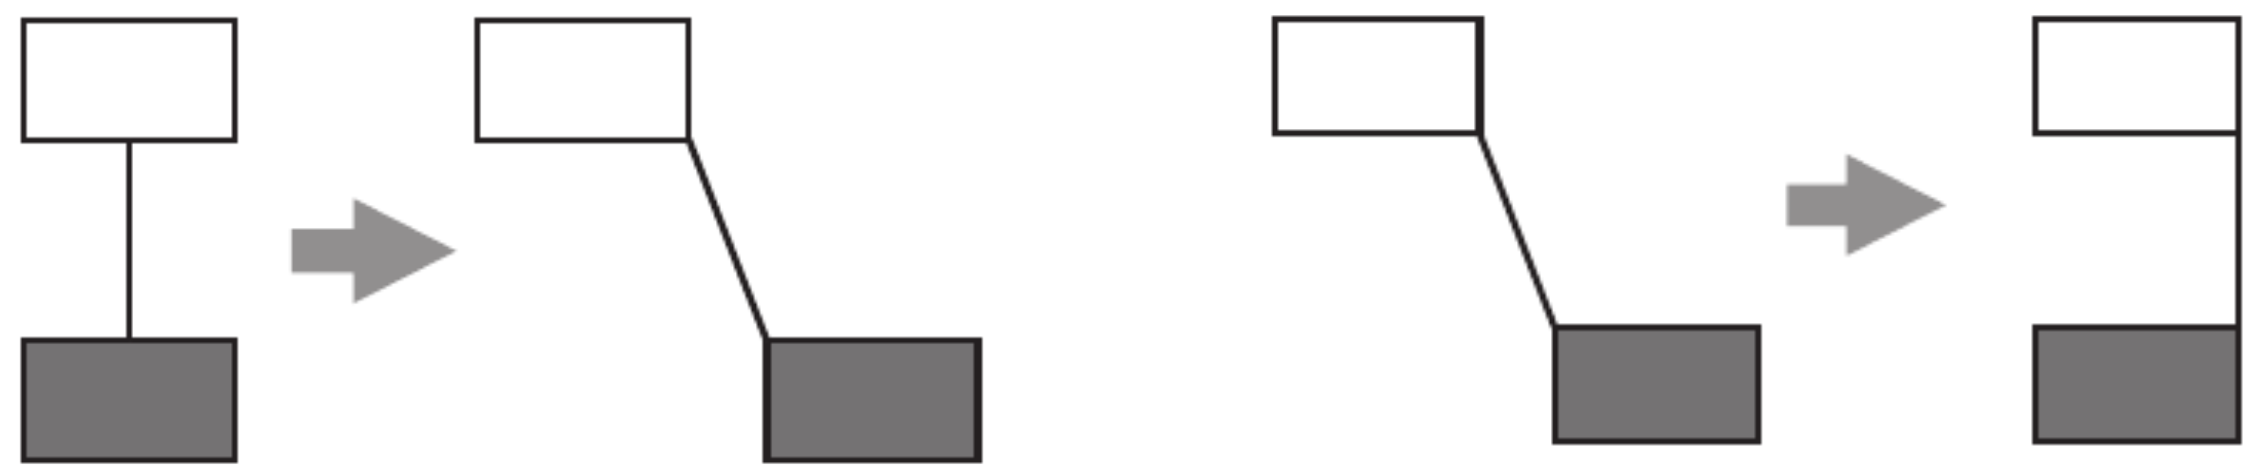
\includegraphics[width=0.8\textwidth]{mementoMotivation.png}
    \attribution{Э. Гамма и др., Приемы объектно-ориентированного проектирования}
\end{center}

Тут фигура честно вернулась в исходное положение, но связь подумала, что фигура просто переместилась, и прицепилась не к тем точкам, что были изначально.

Паттерн <<Хранитель>> описывает более-менее общее решение по хранению всякой информации о состоянии объекта так, чтобы его можно было потом восстановить, и, главное, так, чтобы детали этого состояния не раскрывались сторонним объектам. Например, у нас команда для операции отмены вынуждена знать координаты фигуры, а потом ещё координаты всех связей фигуры, а потом окажется, что и ещё что-то (если вдруг отработал алгоритм автоматического размещения, команде надо знать про координаты вообще всех объектов на сцене). Команде этого всего знать не надо на самом деле, она должна просто получить некое состояние на хранение, а когда ей вызовут Undo(), выдать сохранённое состояние фигуре (или сцене), чтобы те уже сами из него восстановили всё как было. Вот, собственно, этим паттерн <<Хранитель>> и занимается.

\subsection{Хранитель (Memento), общая структура}

Общая структура паттерна такова:

\begin{center}
    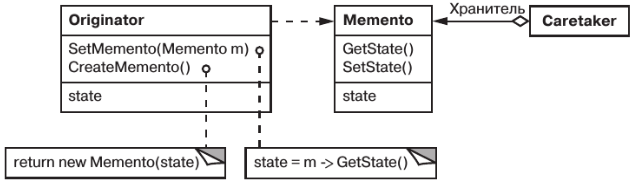
\includegraphics[width=0.7\textwidth]{memento.png}
    \attribution{Э. Гамма и др., Приемы объектно-ориентированного проектирования}
\end{center}

Originator --- это тот, кто хочет сохранить своё состояние и иметь возможность восстановиться из ссохранённой копии. Memento --- это, собственно, сохранённое состояние. Caretaker --- это тот, кто состояние хранит, но не хочет (и не может) лезть внутрь. В нашем примере Caretaker --- это команда, Originator --- это фигура, а Memento --- это класс, прячущий у себя внутри координаты и фигуры, и линий, и всего, что надо.

Когда Caretaker-у нужно сохранить состояние Originator-а, он вызывает метод CreateMemento() и получает некий объект, про который сам Caretaker знает только то, что он есть (state и методы по его управлению он не видит). Когда надо восстановить состояние Originator-а, Caretaker вызывает его метод SetMemento(), Originator (зная конкретный тип Memento) пользуется GetState(), чтобы достать из Memento данные и положить их в свой state.

\subsection{Детали реализации}

В плане реализации это очень простой паттерн, но требующий языковой поддержки. В C++, например, Memento можно сделать friend-классом для Originator-а, в C\# вложеннным классом в Originator, в Java --- статическим вложенным классом. В любом случае, нам нужен механизм, который бы позволял Memento иметь <<широкий>> интерфейс для Originator и <<узкий>> для всех остальных объектов. Чаще всего это требует, чтобы CreateMemento() возвращал абстрактный класс без внутренней структуры (например, Object), а SetMemento() преобразовывал его к нужному типу.

Ещё Memento не обязан хранить всё состояние Originator-а, он может хранить только дельту относительно предыдущего состояния (как бы в обратную сторону, чтобы по текущему можно было получить предыдущее). Тогда, чтобы откатиться к произвольному состоянию, надо иметь список Memento и последовательно их применять. Это экономнее в плане памяти, но гораздо хлопотнее в плане реализации. Например, системы контроля вресий, можно сказать, используют такой подход.

\section{Паттерн <<Интерпретатор>>}

\subsection{Мотивирующий пример}

Паттерн <<Интерпретатор>> используется как легковесная замена полноценных интерпретаторов и компиляторов, когда в программе надо представлять некоторые сложные выражения, уметь их считать и/или делать с ними ещё что-то (например, красиво печатать). Например, разобранное регулярное выражение может храниться в таком виде:

\begin{center}
    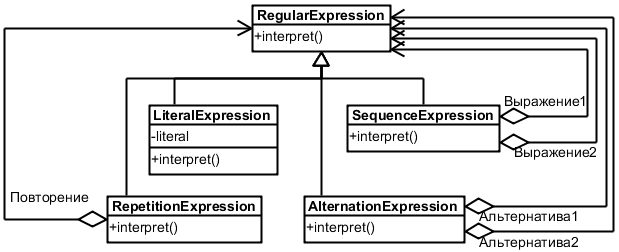
\includegraphics[width=0.85\textwidth]{regexp.png}
\end{center}

На самом деле, это просто абстрактное синтаксическое дерево с операцией interpret(), которая делает какую-то полезную работу (например, проверяет строку на соответствие регулярному выражению).

\subsection{Интерпретатор (Interpreter), общая структура}

Общая схема паттерна такова:

\begin{center}
    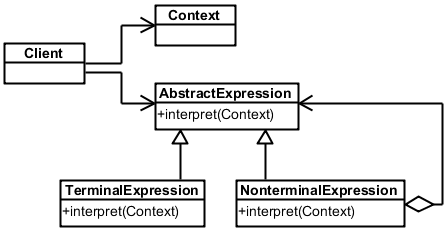
\includegraphics[width=0.65\textwidth]{interpreter.png}
\end{center}

Вообще, это обычное абстрактное синтаксическое дерево (кстати, паттерн <<Компоновщик>>), снабжённое дополнительными операциями, которые могут принимать некий контекст вычислений и что-то делать по этому дереву (например, считать его значение). Пользуется этим делом класс Client. 

В нектором смысле <<Интерпретатор>> --- это прямая противоположность предыдущему паттерну, <<Посетитель>>. Там мы говорили, что операций над сложной структурой данных может быть много и они сами могут быть сложными, так что имеет смысл отделить их в Visitor-ы. Тут же мы говорим, что если структура данных не такая и сложная, операций ограниченное количество и они сами по себе не сильно сложны, то и нечего городить огород, давайте лучше в самих узлах операции реализуем.

При этом паттерн применяется только если структура данных не сложна. Обычно этот паттерн используется для некоторых языков, тогда это можно перефразировать так, что грамматика языка должна быть простой. Для какого-нибудь C\# лучше всё-таки полноценный Visitor. И эффективность не должна быть критична --- <<Интерпретатор>> будет интерпретировать выражение заведомо медленнее, чем скомпилированный код (не то чтобы прямо скомпилированный --- по регулярным выражениям, например, легко построить конечный автомат, который интерпретировать гораздо быстрее и легче, чем дерево разбора регулярного выражения). Поэтому <<Интерпретатор>> используется обычно для реализации маленьких встроенных предметно-ориентированных языков\footnote{Предметно-ориентированный язык называется \emph{встроенным}, если он использует грамматику языка, на котором пишется основная программа (например, можно сделать вполне крутой язык из переопределённых операторов в синтаксисе C++, см., например, boost::spirit), и \emph{внешним}, если у него есть свой компилятор/интерпретатор.}. Кстати, нам дальше встретится паттерн <<Спецификация>> --- это <<Интерпретатор>> конкретно для булевых предикатов.

\subsection{Детали реализации}

Казалось бы, кому нужны маленькие встроенные предметно-ориентированные языки. Однако же есть известное \emph{10-е правило Гринспена}, сформулированное очень давно, поэтому довольно старомодно: <<Любая достаточно сложная программа на Си или Фортране содержит заново написанную, неспецифицированную, глючную и медленную реализацию половины языка Common Lisp>>. В современном мире речь идёт не про Фортран и Лисп, но на практике автора примерно в половине проектов в какой-то момент появлялся какой-то свой самодельный язык, иногда крайне кривой (был даже язык рекурсивного переписывания строк наподобие машин Маркова\footnote{Вычислительно эквивалентный машинам Тьюринга и лямбда-исчислению формализм, чем-то напоминающий формльные грамматики} для генерации контента обучающей системы! Валентин Фёдорович Турчин\footnote{Автор языка Рефал, одного из очень немногих, использующих машины Маркова в качестве модели вычислений} бы одобрил, если бы авторы языка не ограничили глубину стека вызовов числом 42 --- для рекурсивного-то языка). Иногда для таких самодельных языков даже писались IDE-шки. В общем, потребность в таких вещах в индустрии неожиданно высока, так что паттерн <<Интерпретатор>> может не раз пригодиться.

Паттерн не специфицирует посторение дерева. Часто бывает так, что это дерево формирует сам программист, собирая прямо в коде из базовых операций (что-то в духе var businessRule = Add(salary.Data(), bonus.Data());). Иногда дерево получается более автоматически (в т.ч. с помощью паттерна <<Builder>>). Тут всё зависит от конкретной ситуации, так что готовых рецептов нет.

Ещё можно, как обычно в паттерне <<Компоновщик>>, подумать о разделяемых поддеревьях. Терминальные (или листовые) узлы --- это готовые кандидаты для применения паттерна <<Приспособленец>>, потому что у них даже уже есть внешнее состояние (то, что Client передаёт в Context). Однако если дело дошло до паттерна <<Приспособленец>>, дела, скорее всего, уже плохи.

Ну и главное, что надо помнить при реализации паттерна <<Приспособленец>> --- что его, возможно, вообще не надо реализовывать, потому что есть паттерн <<Посетитель>>, решащий похожую задачу (хотя и несколько более общую). Если операций над деревом много, лучше <<Посетитель>>. Если операции сложные и их желательно инкапсулировать (даже если операция одна) --- снова <<Посетитель>>.

\section{Паттерн <<Итератор>>}

\subsection{Итератор (Iterator), общая структура}

<<Итератор>> --- это паттерн, которому не нужен мотивирующий пример, поскольку все наверняка пользовались им ещё с первого курса (даже те, кто программировал только на Си, индекс в массиве суть вариант реализации итератора). <<Итератор>> --- паттерн, который предлагает несколько способов реализации способа обхода некоторой однородной коллекции (массива, списка, дерева, у которого все элементы одного типа, и т.д.). Общая схема итератора такова:

\begin{center}
    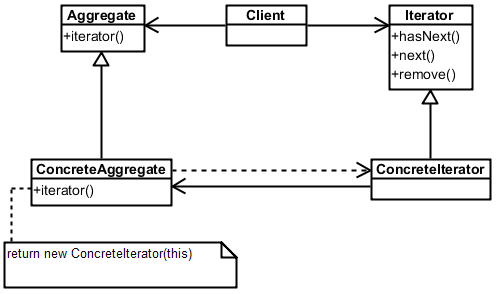
\includegraphics[width=0.7\textwidth]{iterator.png}
\end{center}


Есть коллекция (Aggregate), есть клиент (Client), который хочет её обойти, посетив последовательно все элементы. Для этого он просит у коллекции объект, инкапсулирующий в себе способ обхода, вызовом метода iterator(), и дальше работает с ним, вызывая next(), hasNext()и, при необходимости, remove(). Каждая коллекция может иметь свой специфичный для неё способ обхода (например, очевидно, что дерево обходить надо как-то отлично от списка), поэтому каждая конкретная коллекция (ConcreteAggregate) создаёт свой конкретный итератор (ConcreteIterator), о котором, однако же, клиенту знать не надо, он может обходить коллекцию только с использованием интерфейса Iterator.

Такое устойство позволяет в итераторе полностью <<спрятать>> способ и порядок обхода коллекции, так что можно, например, реализовать обходы в ширину, в глубину, preorder, postorder и т.д. При этом одну и ту же коллекцию могут обходить сколько угодно клиентов и сколькими угодно способами одновременно. А можно обходить и не коллекции, а вообще любую структуру данных, где есть понятие <<следующий элемент>> (например, поток событий с датчиков), или даже генерировать данные <<на ходу>> (например, итератор может представлять бесконечную последовательность простых чисел, которую он сам же и генерирует).

\subsection{Детали реализации}

<<Итератор>>, несмотря на то, что один из самых известных паттернов проектирования, имеет массу тонкостей реализации. Человечество даже не смогло договориться об единой форме интерфейса итератора, поэтому в стандартных библиотеках популярных языков есть два разных стиля. Java-стиль:

\begin{minted}{java}
public interface Iterator<E> {
    boolean hasNext();
    E next();
    void remove();
}
\end{minted}

Метод next() тут возвращает текущий элемент коллекции и продвигает итератор на следующий, а hasNext() говорит, есть ли следующий вообще. В Java итератор также имеет метод remove() для удаления текущего элемента из коллекции, но большинство коллекций его не реализуют.

.NET-стиль (на самом деле, скорее C++-стиль):

\begin{minted}{csharp}
public interface IEnumerator<T>
{
    bool MoveNext();
    T Current { get; }
    void Reset();
}
\end{minted}

Здесь Current возвращает текущий элемент коллекции, а MoveNext() продвигается на следующий (и возвращает false, если его нет). Reset() возвращает итератор в начальное положение --- перед первым элементом коллекции (то есть сначала надо сделать MoveNext, затем Current). 

В общем-то, оба стиля итераторов делают одно и то же и одинаково удобны на практике, разве что итератор из Java немного более удобен для обхода циклом for, а .NET-стиль --- для ручного управления обходом, но различия очень незначительны. Тем более что всё равно современные языки прячут итераторы за синтаксическим сахаром типа циклов foreach.

Ещё в библиотеках часто встречаются \emph{внешшние} и \emph{внутренние} итераторы. Внешний итератор позволяет клиенту определять, когда переходить на следующий элемент, внутренний --- колелкции передаётся действие, которое надо выполнить над всеми её элементами, и она сама себя обходит (она сама создаёт итератор и обходит им, если точнее), вызывая действие. Пример внешнего итератора в .NET --- это интерфейс IEnumerator из примера выше, у которого при желании можно вызывать MoveNext вручную, но обычно он используется в цикле foreach:

\begin{minted}{csharp}
foreach (Thing t in collection)
{
    Console.WriteLine(t);
} 
\end{minted}

Тут компилятор сам генерирует код, который создаёт итератор от collection и делает MoveNext() на каждой итерации, присваивая Current переменной t. На самом деле, он ещё и оборачивает это всё в try-catch, чтобы корректно финализировать итератор (итератор вполне может ходить по коллекции в базе данных, так что должен иметь возможность закрыть соединение даже в случае, если всё плохо).

Внутренний итератор в .NET же используется вот так:

\begin{minted}{csharp}
collection.ToList().ForEach(t => Console.WriteLine(t));
\end{minted}

\mintinline{csharp}{t => Console.WriteLine(t)} --- это лямбда-функция от одного аргумента (t), которая вызывается для каждого элемента коллекции collection. И, в данном случае, печатает его на экран. Тут все MoveNext-ы и Current-ы спрятаны внутрь коллекции, и на самом деле она вправе ими вообще не пользоваться, а реализовать обход как угодно (хотя конкретно в .NET это всё равно реализуется через IEnumerator). Кстати, обратите внимание, что в .NET <<итератор>> называется <<энумератор>>, потому что немного отличается от того, что в Java, и чтобы программисты не путались.

Внешние итераторы хороши тем, что дают большую гибкость и позволяют обходить коллекцию несколькими инетароами согласованно (например, в сортировке слиянием надо совместно обходить два массива, выбирая из них наименьший элемент). Внутренние итераторы хороши тем, что проще в использовании, поэтому когда нам не надо ничем управлять, а надо просто посетить каждый элемент коллекции, они удобней.

Ещё на самом деле есть более концептуально простая штука, чем итератор, называется \emph{курсор}. Это структура, которая содержит в себе данные о текущем положении в коллекции, и коллекция может продвигать курсор на следующую позицию или возвращать текущее значение по курсору. Например, курсором может быть индекс в массиве или указатель на текущий элемент списка. В отличие от итератора, при использовании курсора логика обхода реализуется в самой коллекции, но всё так же можно обходить одну коллекцию несколькими курсорами одновременно и возможна даже реализация разных вариантов обхода. Однако используются курсоры реже, поскольку не так удобны, как итераторы (в частности, надо хранить ссылку на коллекцию, без неё курсор бесполезен).

Ещё итераторы делятся на \emph{устойчивые} и \emph{неустойчивые}. Устойчивые итераторы могут корректно продолжить обход коллекции, если коллекция поменялась. Неустойчивые при любом изменении коллекции прекращают обход и выдают ошибку при попытке получения следующего элемента. Казалось бы, устойчивые итераторы удобнее, но в бибилотеках абсолютное большинство итераторов неустойчивые. Потому что они гораздо проще в реализации и имеют понятную семантику. Устйчивые итераторы обычно требуют механизм, при котором коллекция нотифицирует их об изменениях (например, паттерном <<Наблюдатель>>). 

Однако неустойчивые итераторы тоже не так просты, как кажутся --- они тоже должны понять, что коллекция изменилась, чтобы корректно поругаться, а не продолжать обход как попало. Это делается проще всего с помощью версий коллекции --- если в ней что-то меняется, она увеличивает на один свою версию (которая хранится просто как целочисленное поле). Итератор при выполнении любой операции сверяет сохранённую в  момент своего создания версию с текущей версией коллекции, и если они отличаются, то кидает исключение. Например, итератор в .NET кидает исключение, что коллекция модифицирована, при выполнении MoveNext(), однако гарантирует успешное выполнение Current всегда --- даже если элемент, на который указывает итератор, был удалён. Reset() тоже можно делать, если коллекция изменилась. 

Обычно итераторы имеют очень простой интерфейс (два примера, для Java и для .NET приведены выше), он зафиксирован в стандартной библиотеке и ему следуют все итераторы всех коллекций. Кстати, обычно этот интерфейс используется в паре с интерфейсом <<то, у чего есть итератор>> (Iterable в Java или \mintinline{csharp}{IEnumerable<T>} в .NET), со всего одним методом <<получить итератор>> (тоже общим для всех коллекций и не только коллекций). Однако иногда могут требоваться и дополнительыне операции, например, итераторы, способные ходить по коллекции в обе стороны, итераторы с эффективным произвольным доступом по индексу и т.д. Обычно они реализуются как наследники стандартного интерфейса, но в реальной жизни встречаются довольно редко, потому что на самом деле в 99 процентах случаев достаточно просто по коллекции пройти, без всяких излишеств. Исключение --- C++, где в стандартной библиотеке очень развитый механизм поддержки разных сортов итераторов. Однако он настолько сложен, что одно время в boost (очень популярной дополнительной библиотеке для C++) был механизм проверки итератора на корректность --- потому что выяснилось, что даже опытные программисты не всегда пишут правильные с точки зрения различных ограничений и договорённостей стандартной библиотеки итераторы с первого раза. А неправильный итератор мог приводить к малозаметным багам в стандартных алгоритмах, которые им пользуются. В общем, в современных языках итераторы просты, и это прекрасно.

\end{document}